\blankpage

\pagestyle{hedra}
\label{hedra}
%\begin{textblock*}{5.625in}(0pt,0pt)%
%\vspace*{-3.5cm}
%\hspace*{-2.77cm}\includegraphics*[width=175.2mm]{./propagandas/HEDRA.pdf}
%\end{textblock*}
%\pagebreak

\begin{center}
\hspace*{-3.6cm}\raisebox{5cm}{\rotatebox[origin=t]{90}{\huge\textbf{Lançamento}}}
\hspace*{3.1cm}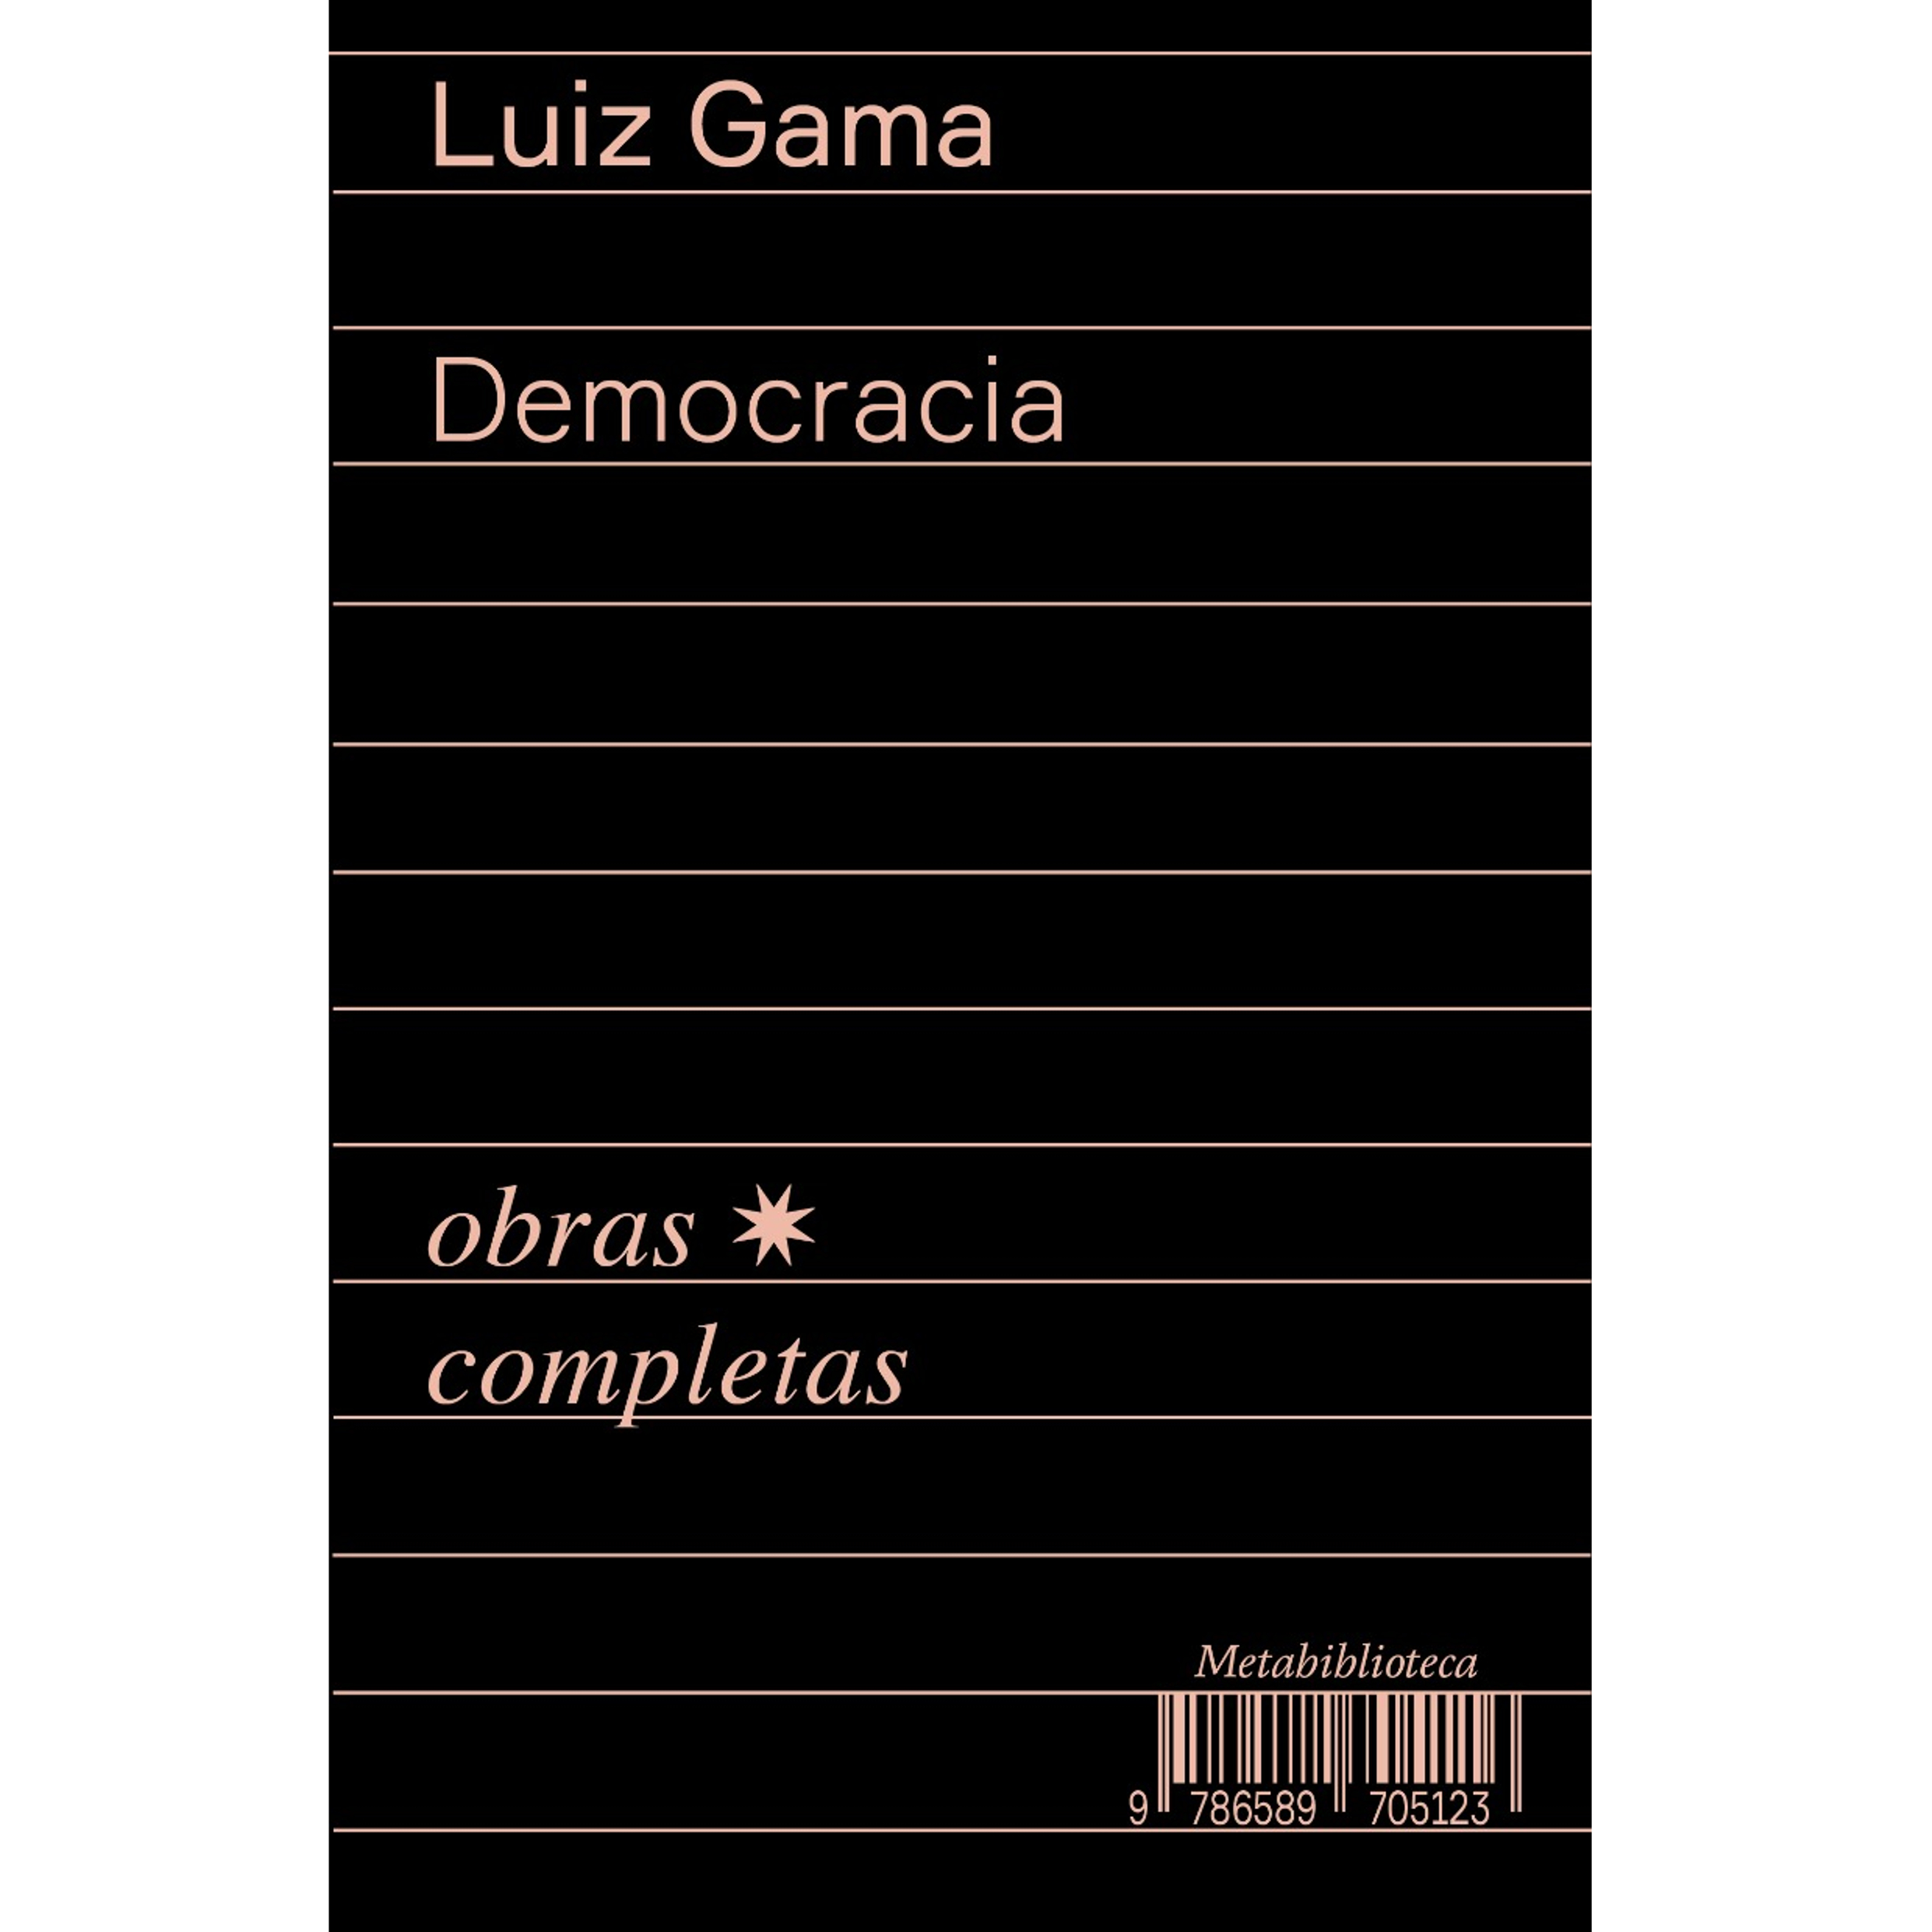
\includegraphics[width=74mm]{./CAPAS/HEDRA_DEMOCRACIA.jpg}
\end{center}
\hspace*{-7cm}\hrulefill\hspace*{-7cm}
\medskip

\noindent{}Os textos e artigos incluídos em \textit{Democracia} foram publicados originalmente entre os anos de 1866 e 1869. Nesses artigos, Luiz Gama se manifesta publicamente sobre educação, política e direitos universais. \hlc{Lançando mão de uma estratégia autoral ousada, que incluía o uso de pseudônimos, Gama defende abertamente o direito à educação universal e as obrigações do Estado em garantir um ensino público de qualidade} em todos os níveis como os fundamentos da vida democrática.

\textit{Democracia} integra as \textit{Obras completas} de Luiz Gama, advogado negro e abolicionista, a serem lançadas em 11 volumes com cerca de 800 escritos --- 600 inéditos ---, revelando as diversas facetas e estilos empregados pelo escritor para advogar pela grande causa de sua vida: a abolição da escravidão e a emancipação negra. Esquecidos em parte por quase dois séculos, os textos foram recuperados pelo pesquisador Bruno Rodrigues de Lima, que passou nove anos localizando-os em arquivos da imprensa e do judiciário de todo o país.

\vfill
\noindent\begin{minipage}[c]{1\linewidth}
{\small\textbf{
\hspace*{-.1cm}Editora: Hedra\\
Título: Democracia (1866--1869)\\
Autor: Luiz Gama\\ 
ISBN: 978-65-89705-12-3\\
Páginas: 506\\
Formato: 13,3x21\,cm\\
Preço: R\$ 110,00\\
}}
\end{minipage}
\pagebreak

\begin{center}
\hspace*{.5cm}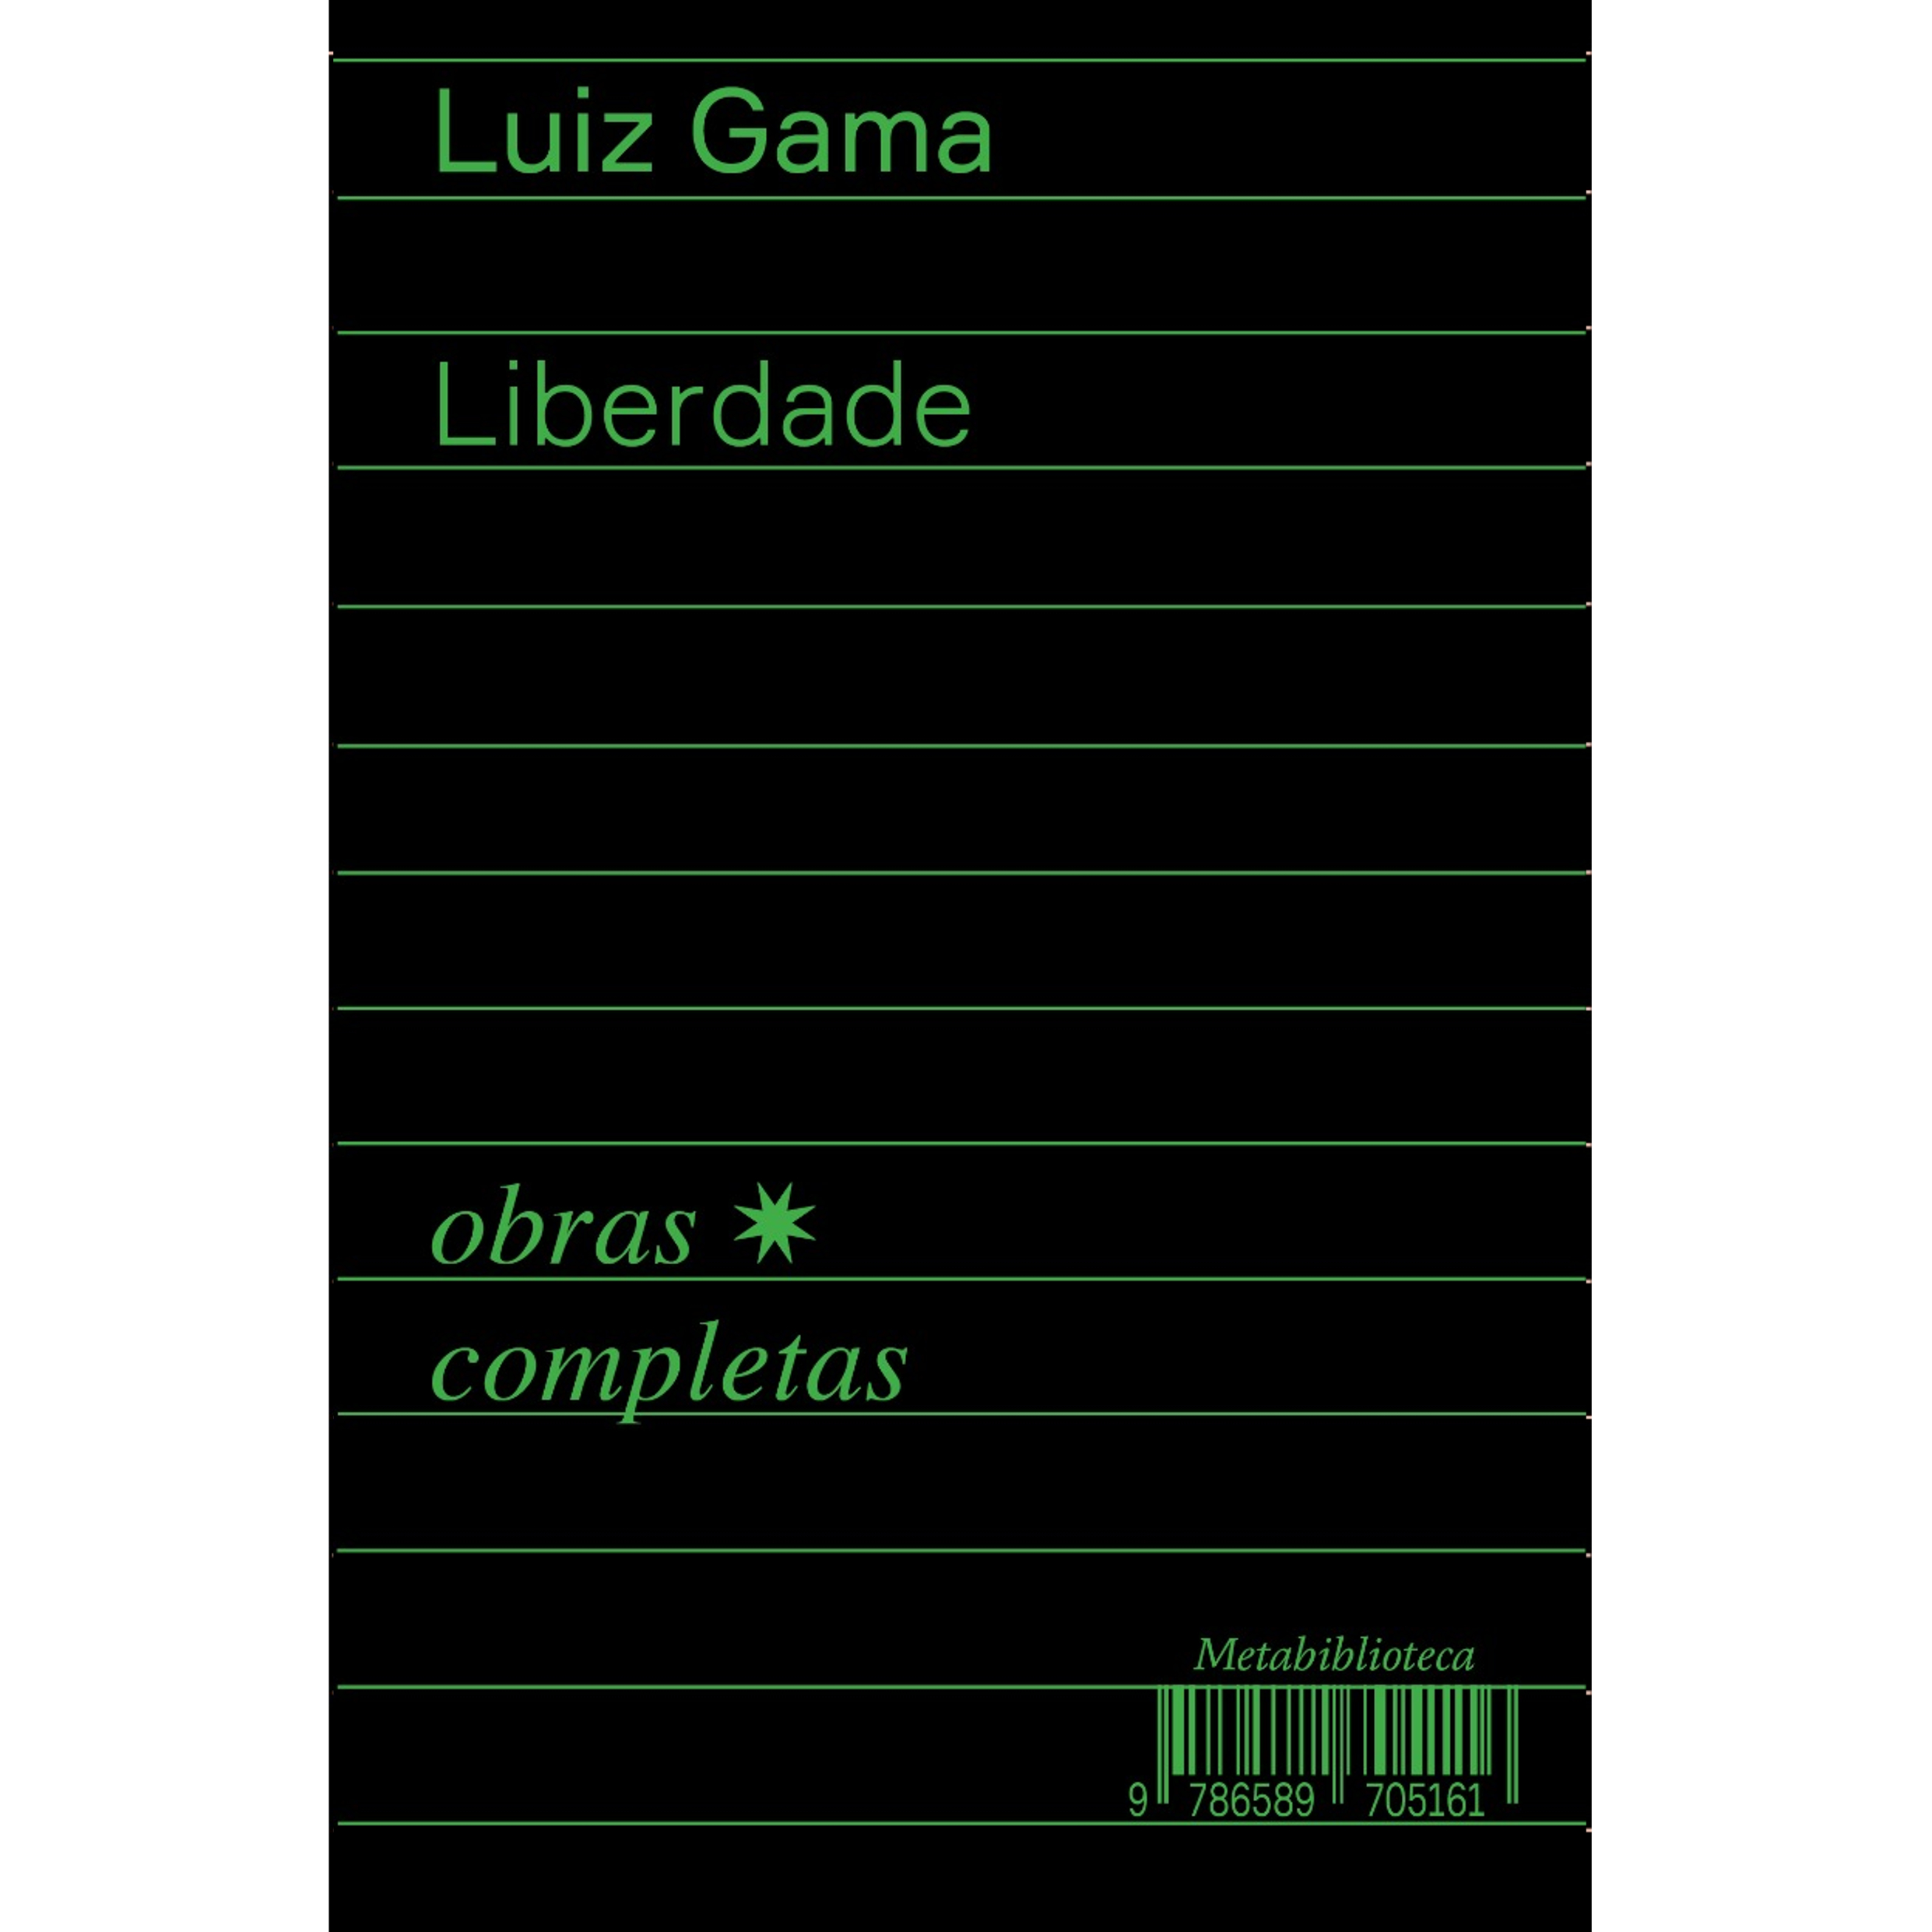
\includegraphics[width=74mm]{./CAPAS/HEDRA_LIBERDADE.jpg}
\end{center}
\hspace*{-7cm}\hrulefill\hspace*{-7cm}
\medskip

\noindent{}Os textos deste volume são \hlc{fruto da campanha pela abolição radical, que também visava à garantia da educação e cidadania para os libertos: o abolicionismo de Gama exigia cidadania e igualdade de fato e de direito}. O advogado também refletia sobre o processo histórico em curso, e propunha soluções políticas para o tempo presente, revelando sua natureza intelectual até hoje pouco conhecida e quase sempre não reconhecida.

\textit{Liberdade} integra as \textit{Obras completas} de Luiz Gama, advogado negro e abolicionista, a serem lançadas em 11 volumes com cerca de 800 escritos --- 600 inéditos ---, revelando as diversas facetas e estilos empregados pelo escritor para advogar pela grande causa de sua vida: a abolição da escravidão e a emancipação negra. Esquecidos em parte por quase dois séculos, os textos foram recuperados pelo pesquisador Bruno Rodrigues de Lima, que passou nove anos localizando-os em arquivos da imprensa e do judiciário de todo o país.

\vfill
\noindent\begin{minipage}[c]{.5\linewidth}
{\small\textbf{
\hspace*{-.1cm}Editora: Hedra\\
Título: Liberdade (1880--1882)\\
Autor: Luiz Gama\\ 
ISBN: 978-65-89705-16-1\\
Páginas: 446\\
Formato: 13,3x21\,cm\\
Preço: R\$ 99,90\\
}}
\end{minipage}
\pagebreak

\begin{center}
\hspace*{-3.6cm}\raisebox{5cm}{\rotatebox[origin=t]{90}{\huge\textbf{Lançamento}}}
\hspace*{3.1cm}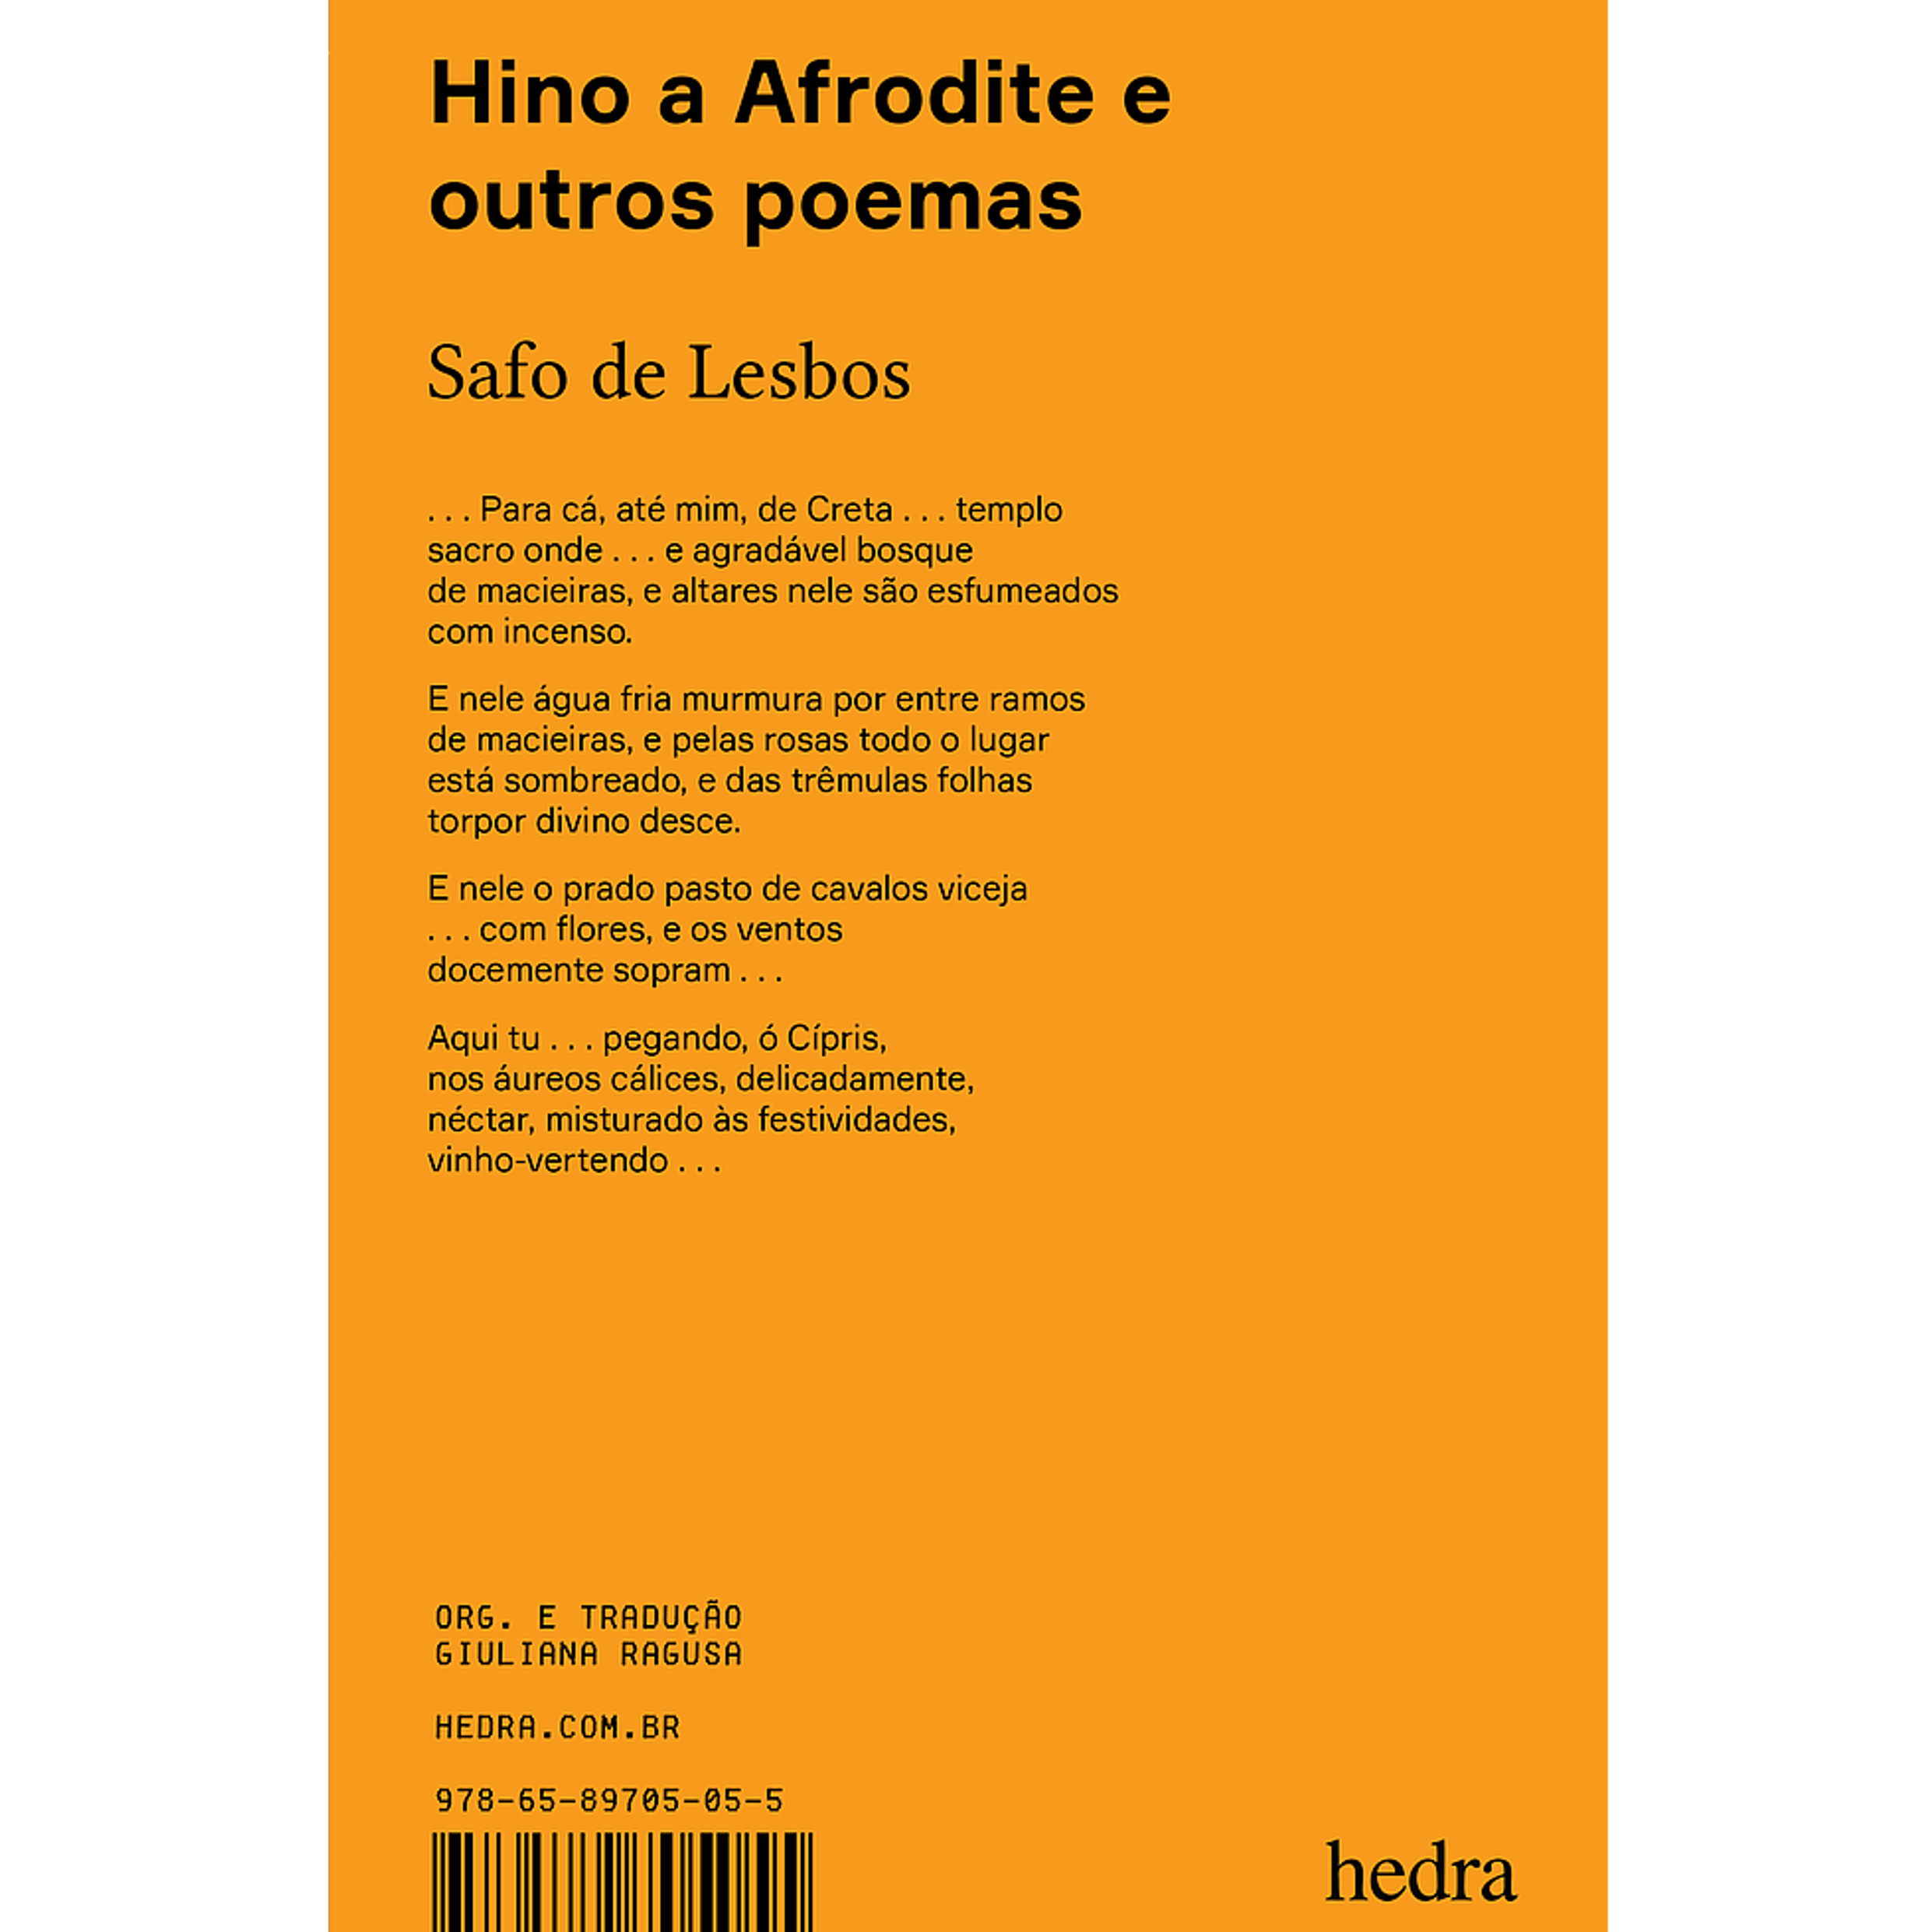
\includegraphics[width=74mm]{./CAPAS/HEDRA_SAFO.jpg}
\end{center}
\hspace*{-7cm}\hrulefill\hspace*{-7cm}
\medskip

\noindent{}Reunião de \hlc{textos remanescentes da mélica de Safo, ou seja, as canções para performance ao som da lira. Os textos aqui são traduzidos e anotados por Giuliana Ragusa em segunda edição --- com novos poemas, atualizações e em versão bilíngue} ---, autora que ganhou o Jabuti 2006 com um livro sobre a lírica da poeta, a única mulher entre os grandes da época. Para esta edição foram selecionados a única canção completa e os fragmentos mais legíveis de canções do corpus de Safo. As anotações de leitura buscam lançar luz sobre elementos relevantes da estrutura, conteúdo ou transmissão dos fragmentos organizados tematicamente. Precede a tradução anotada uma introdução sobre a poeta, sua poesia e o contexto em que se produziu e circulou, o gênero mélico, a fortuna crítica sobre ela, a transmissão de sua obra, e as outras poetas mulheres de que se tem notícia.

\vfill
\noindent\begin{minipage}[c]{1\linewidth}
{\small\textbf{
\hspace*{-.1cm}Editora: Hedra\\
Título: Hino a Afrodite e outros poemas\\
Autor: Safo de Lesbos\\ 
ISBN: 978-65-89705-05-5\\
Páginas: 212\\
Formato: 13,3x21\,cm\\
Preço: R\$ 69,00\\
}}
\end{minipage}
\pagebreak

\begin{center}
\hspace*{.5cm}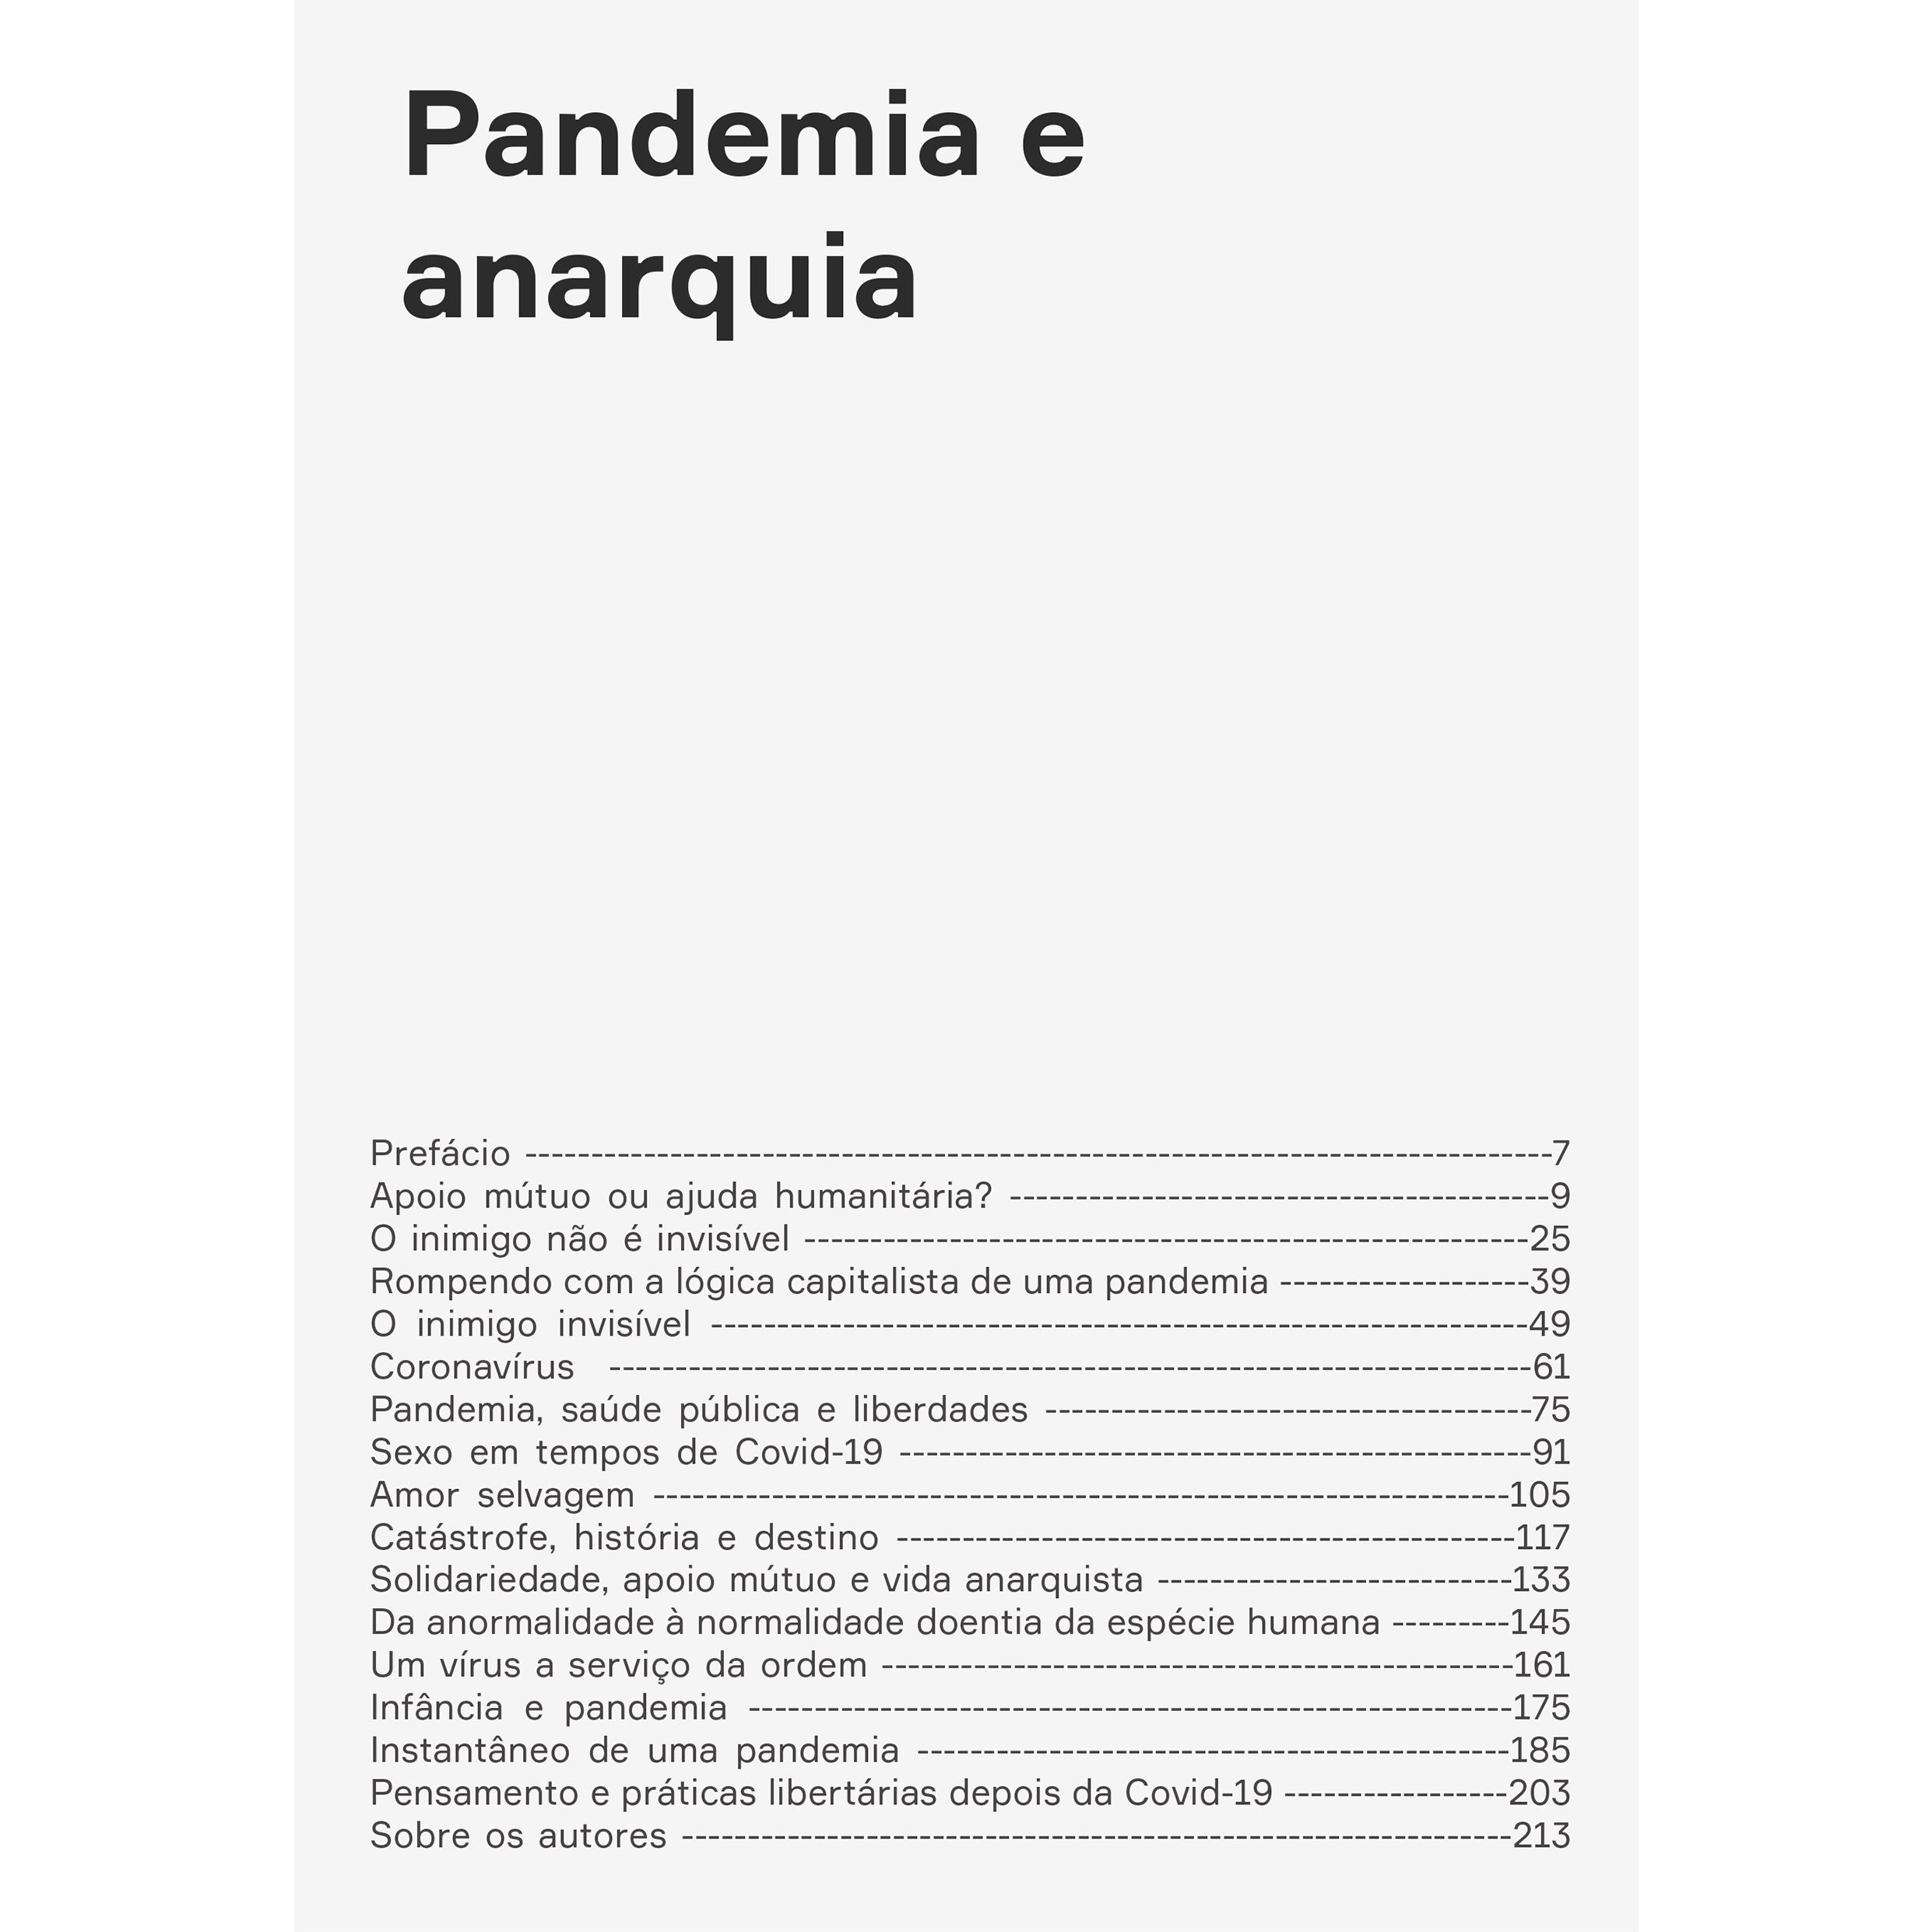
\includegraphics[width=74mm]{./CAPAS/HEDRA_PANDEMIA.jpg}
\end{center}
\hspace*{-7cm}\hrulefill\hspace*{-7cm}
\medskip

\noindent{}\textit{Pandemia e anarquia} reúne quinze ensaios de pesquisadores das práticas libertárias que analisam as implicações sociopolíticas do novo coronavírus e sua relação com os modos de existência. Além da Somaterapia e de pesquisadores do Nu-Sol (Núcleo de Sociabilidade Libertária), este livro traz escritos de historiadores e cientistas políticos residentes em diversos espaços do planeta. \hlc{Perpassando diversas esferas das relações humanas, da economia e da ciência às relações amorosas e ao ser criança durante a pandemia, os escritos insurgem-se contra a suposta ruptura com o mundo dado antes da Covid-19 para analisar e estancar a racionalidade neoliberal}, e a chamada crise sanitária. Com isso, traçam a afirmação de uma vida outra no presente.

\vfill
\noindent\begin{minipage}[c]{.5\linewidth}
{\small\textbf{
\hspace*{-.1cm}Editora: Hedra\\
Título: Pandemia e anarquia\\
Autor: Edson Passetti, João da Mata e José Maria Carvalho Ferreira (orgs.)\\ 
ISBN: 978-65-89705-04-8\\
Páginas: 220\\
Formato: 16x23\,cm\\
Preço: R\$ 69,00\\
}}
\end{minipage}
\pagebreak

\begin{center}
\hspace*{-3.6cm}\raisebox{5cm}{\rotatebox[origin=t]{90}{\huge\textbf{Lançamento}}}
\hspace*{3.1cm}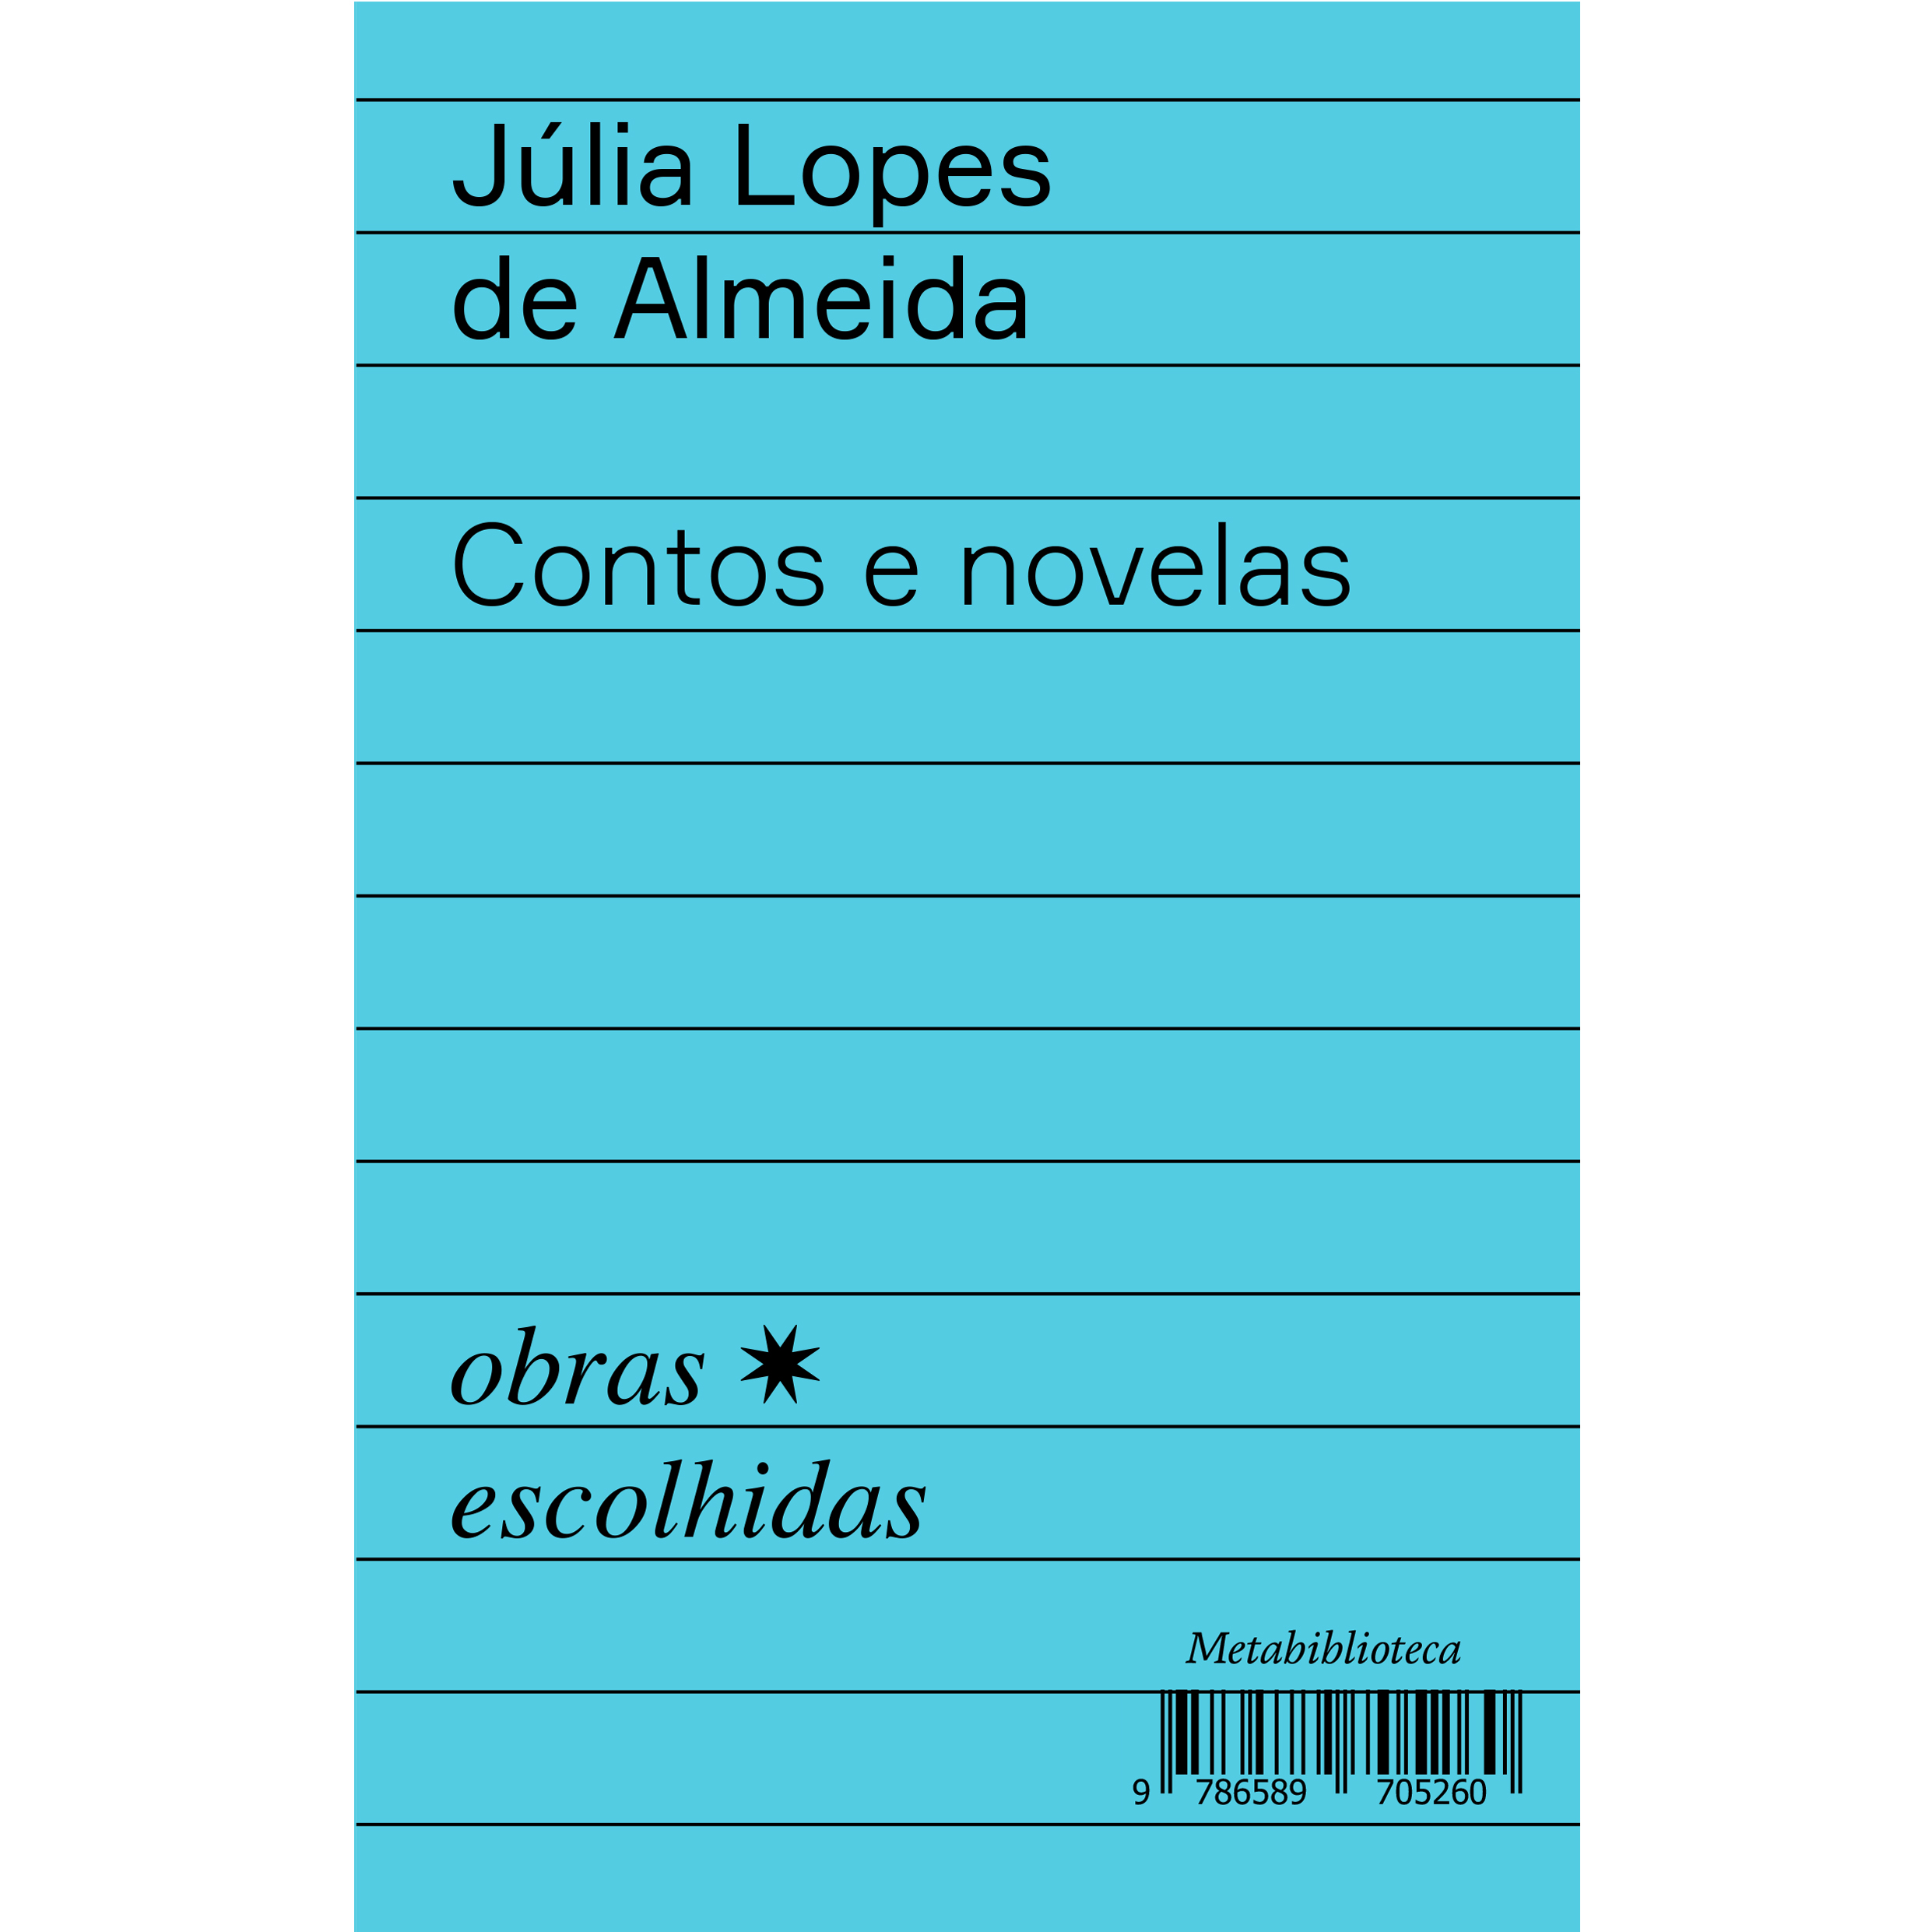
\includegraphics[width=74mm]{./CAPAS/HEDRA_JULIA.jpg}
\end{center}
\hspace*{-7cm}\hrulefill\hspace*{-7cm}
\medskip

\noindent{}\textit{Contos e novelas} reúne narrativas curtas de Júlia Lopes de Almeida, extraídas de duas de suas obras: \textit{Ânsia eterna} (1903) e \textit{A isca} (1922). Da primeira, fortemente influenciada pelo escritor francês Guy de Maupassant, foram selecionados dez contos, marcados pelo insólito e pelo fantástico. Da segunda, que reunia originalmente quatro novelas, foram selecionadas duas que apresentam algumas das características da narrativa de Júlia Lopes e dos temas que permeiam sua obra. \hlc{Com tintas do naturalismo e do realismo francês, sua prosa tem traços da objetividade, do antropocentrismo e do cientificismo que fizeram escola no século XIX. Não ficam de fora, no entanto, as críticas à sociedade brasileira}: o lugar da mulher na sociedade patriarcal, os conflitos familiares, as marcas da escravidão e os contrastes sociais, políticos e econômicos resultantes da modernização são temas recorrentes.

\vfill
\noindent\begin{minipage}[c]{1\linewidth}
{\small\textbf{
\hspace*{-.1cm}Editora: Hedra\\
Título: Contos e novelas: obras escolhidas\\
Autor: Júlia Lopes de Almeida\\ 
ISBN: 978-65-89705-26-0\\
Páginas: 190\\
Formato: 13,3x21\,cm\\
Preço: R\$ 64,00\\
}}
\end{minipage}
\pagebreak

\begin{center}
\hspace*{.5cm}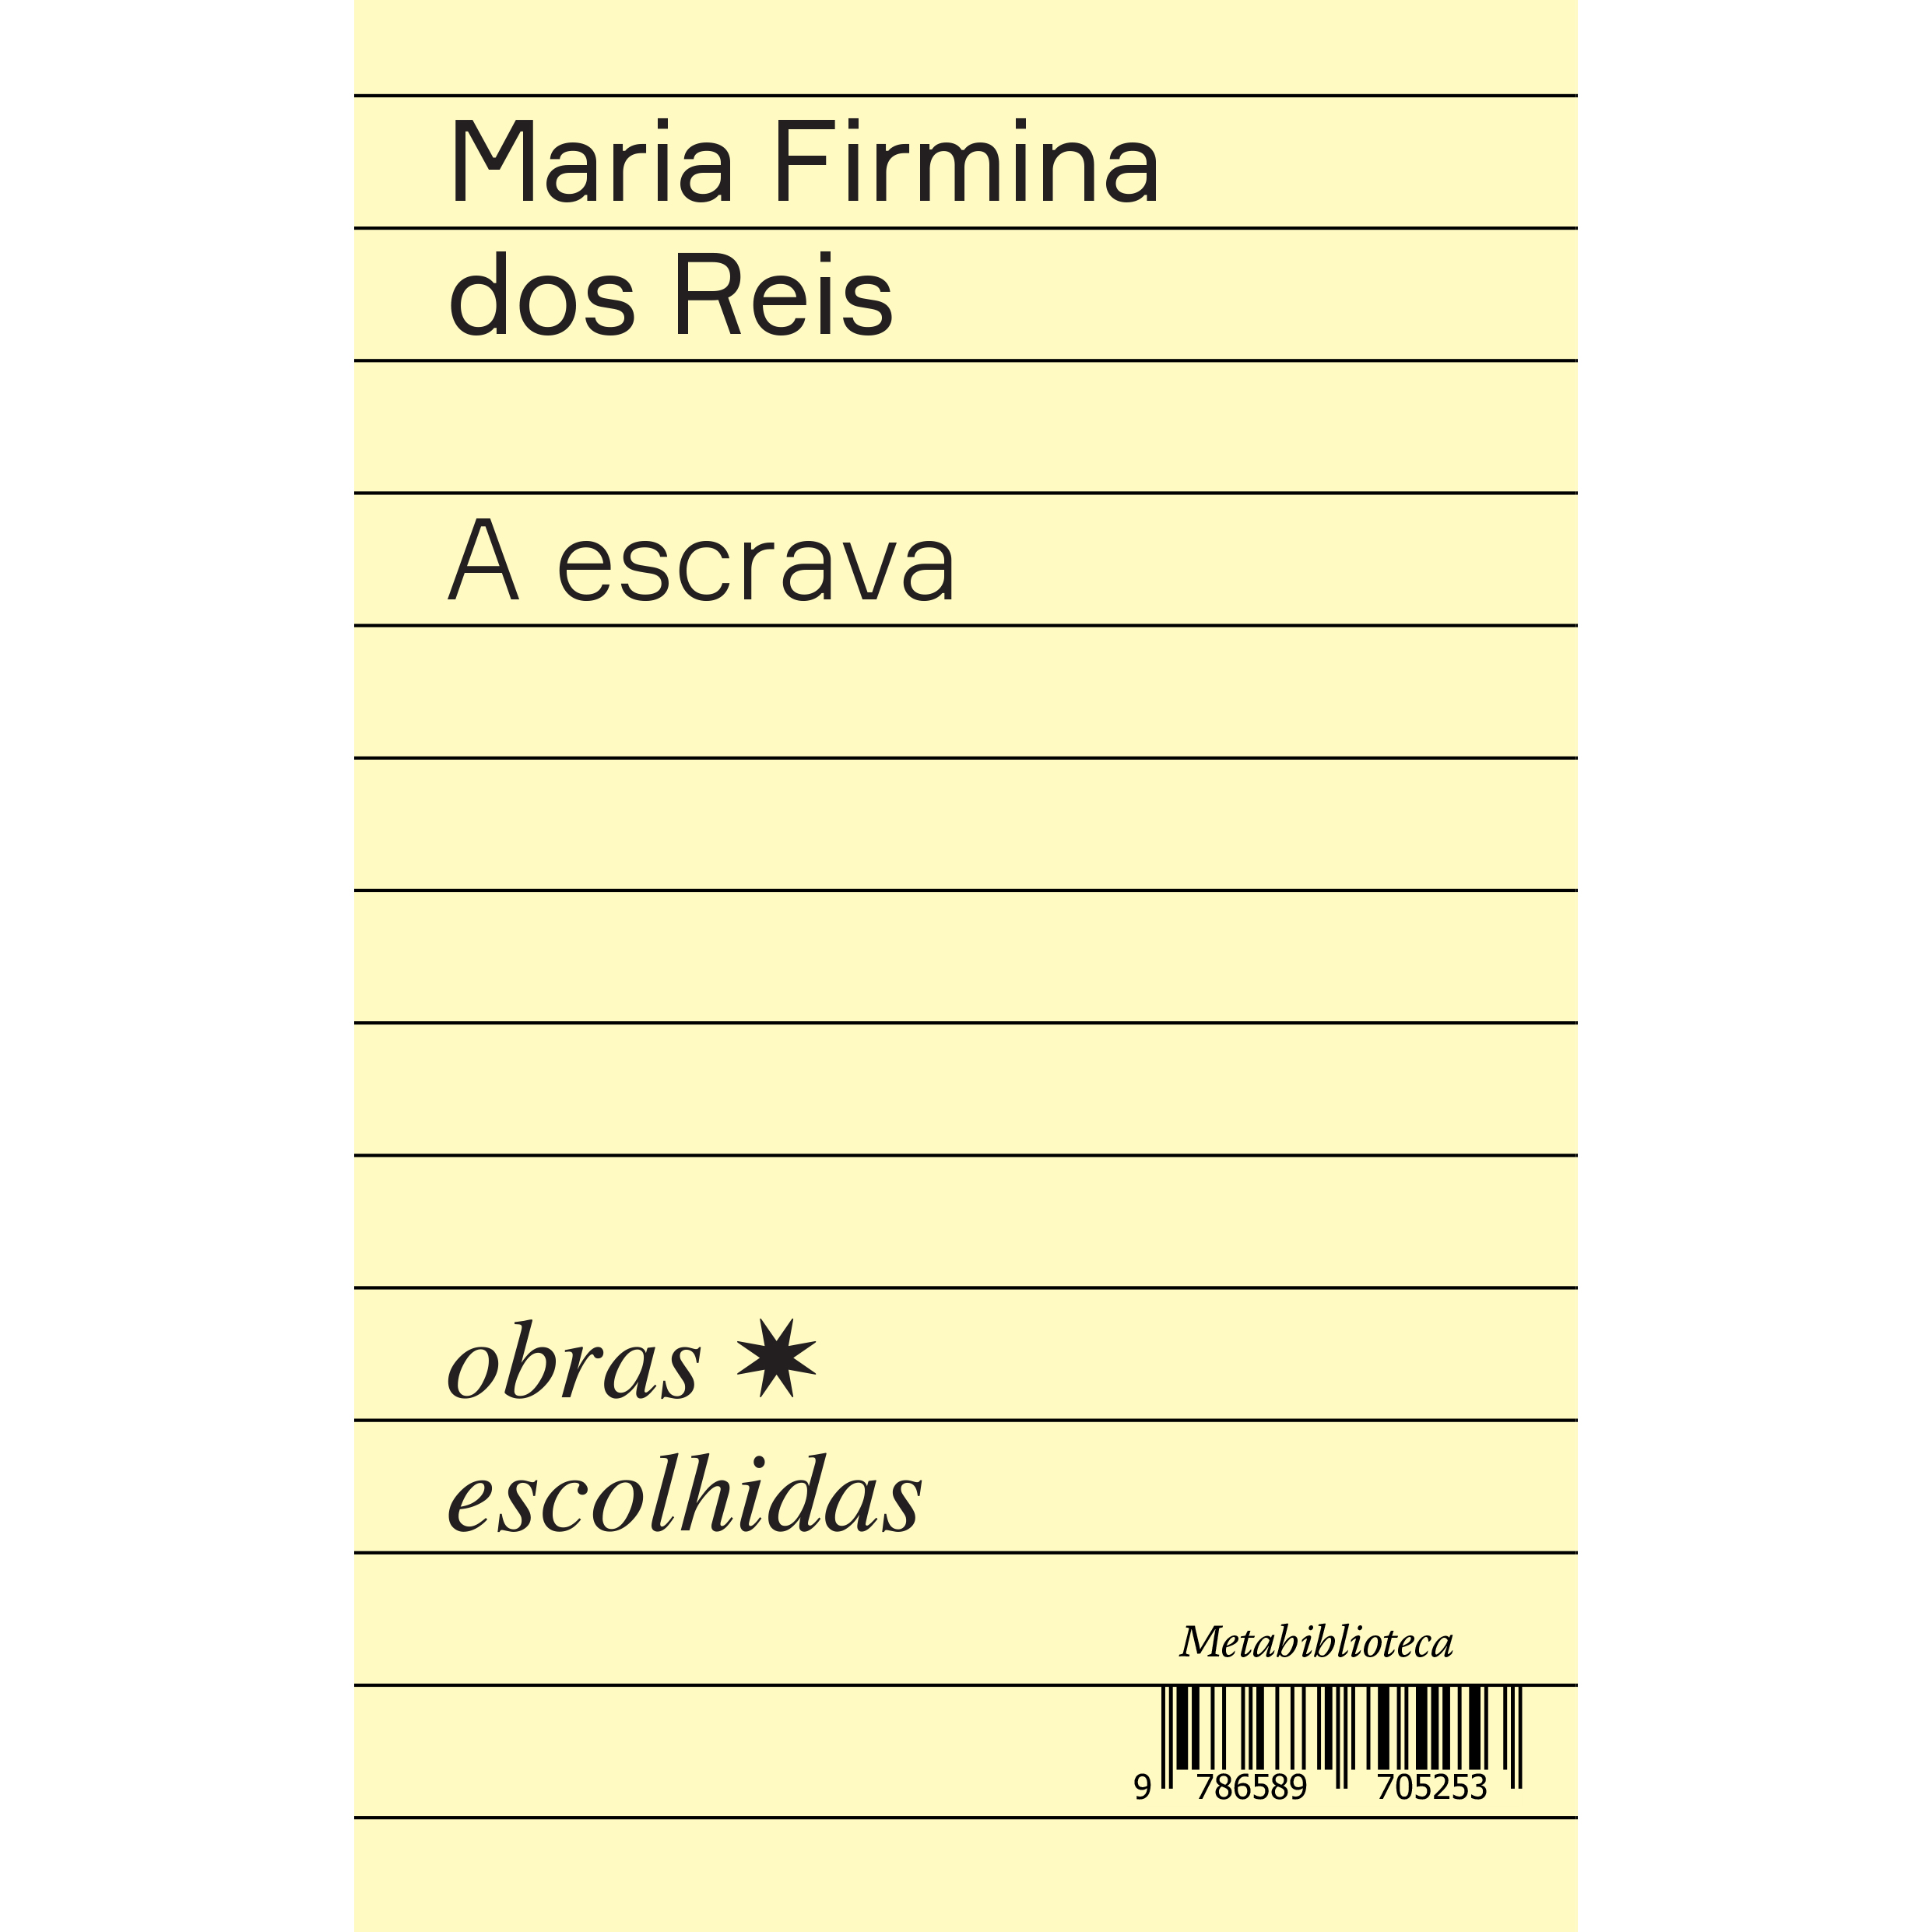
\includegraphics[width=74mm]{./CAPAS/HEDRA_FIRMINA.jpg}
\end{center}
\hspace*{-7cm}\hrulefill\hspace*{-7cm}
\medskip

\noindent{}\textit{A escrava} consiste em uma seleção de textos em prosa e poemas de Maria Firmina dos Reis (1822–1917), considerada a primeira romancista negra da história da literatura brasileira. Estão presentes o conto ``A escrava'', de 1887, a novela ``Gupeva'', de 1861, e 32 poemas: dos quais 29 foram extraídos entre os 56 de \textit{Cantos à beira-mar} (1871), dois da antologia \textit{Parnaso maranhense} (1861), e o famoso ``Hino à liberdade dos escravos'', originalmente escrito para ser cantado e acompanhado por instrumentos musicais. Nesta seleção, apresentam-se alguns dos \hlc{principais elementos que caracterizam a literatura da escritora: a situação dos escravizados, que passam a ter protagonismo nas narrativas, o papel da mulher na sociedade, as condições dos povos indígenas, um sentimentalismo romântico amoroso e a exaltação da terra.}

\vfill
\noindent\begin{minipage}[c]{1\linewidth}
{\small\textbf{
\hspace*{-.1cm}Editora: Hedra\\
Título: A escrava: antologia de prosa e versos\\
Autor: Maria Firmina dos Reis\\ 
ISBN: 978-65-89705-25-3\\
Páginas: 162\\
Formato: 13,3x21\,cm\\
Preço: R\$ 56,00\\
}}
\end{minipage}
\pagebreak

\begin{center}
\hspace*{-3.6cm}\raisebox{5cm}{\rotatebox[origin=t]{90}{\huge\textbf{Lançamento}}}
\hspace*{3.1cm}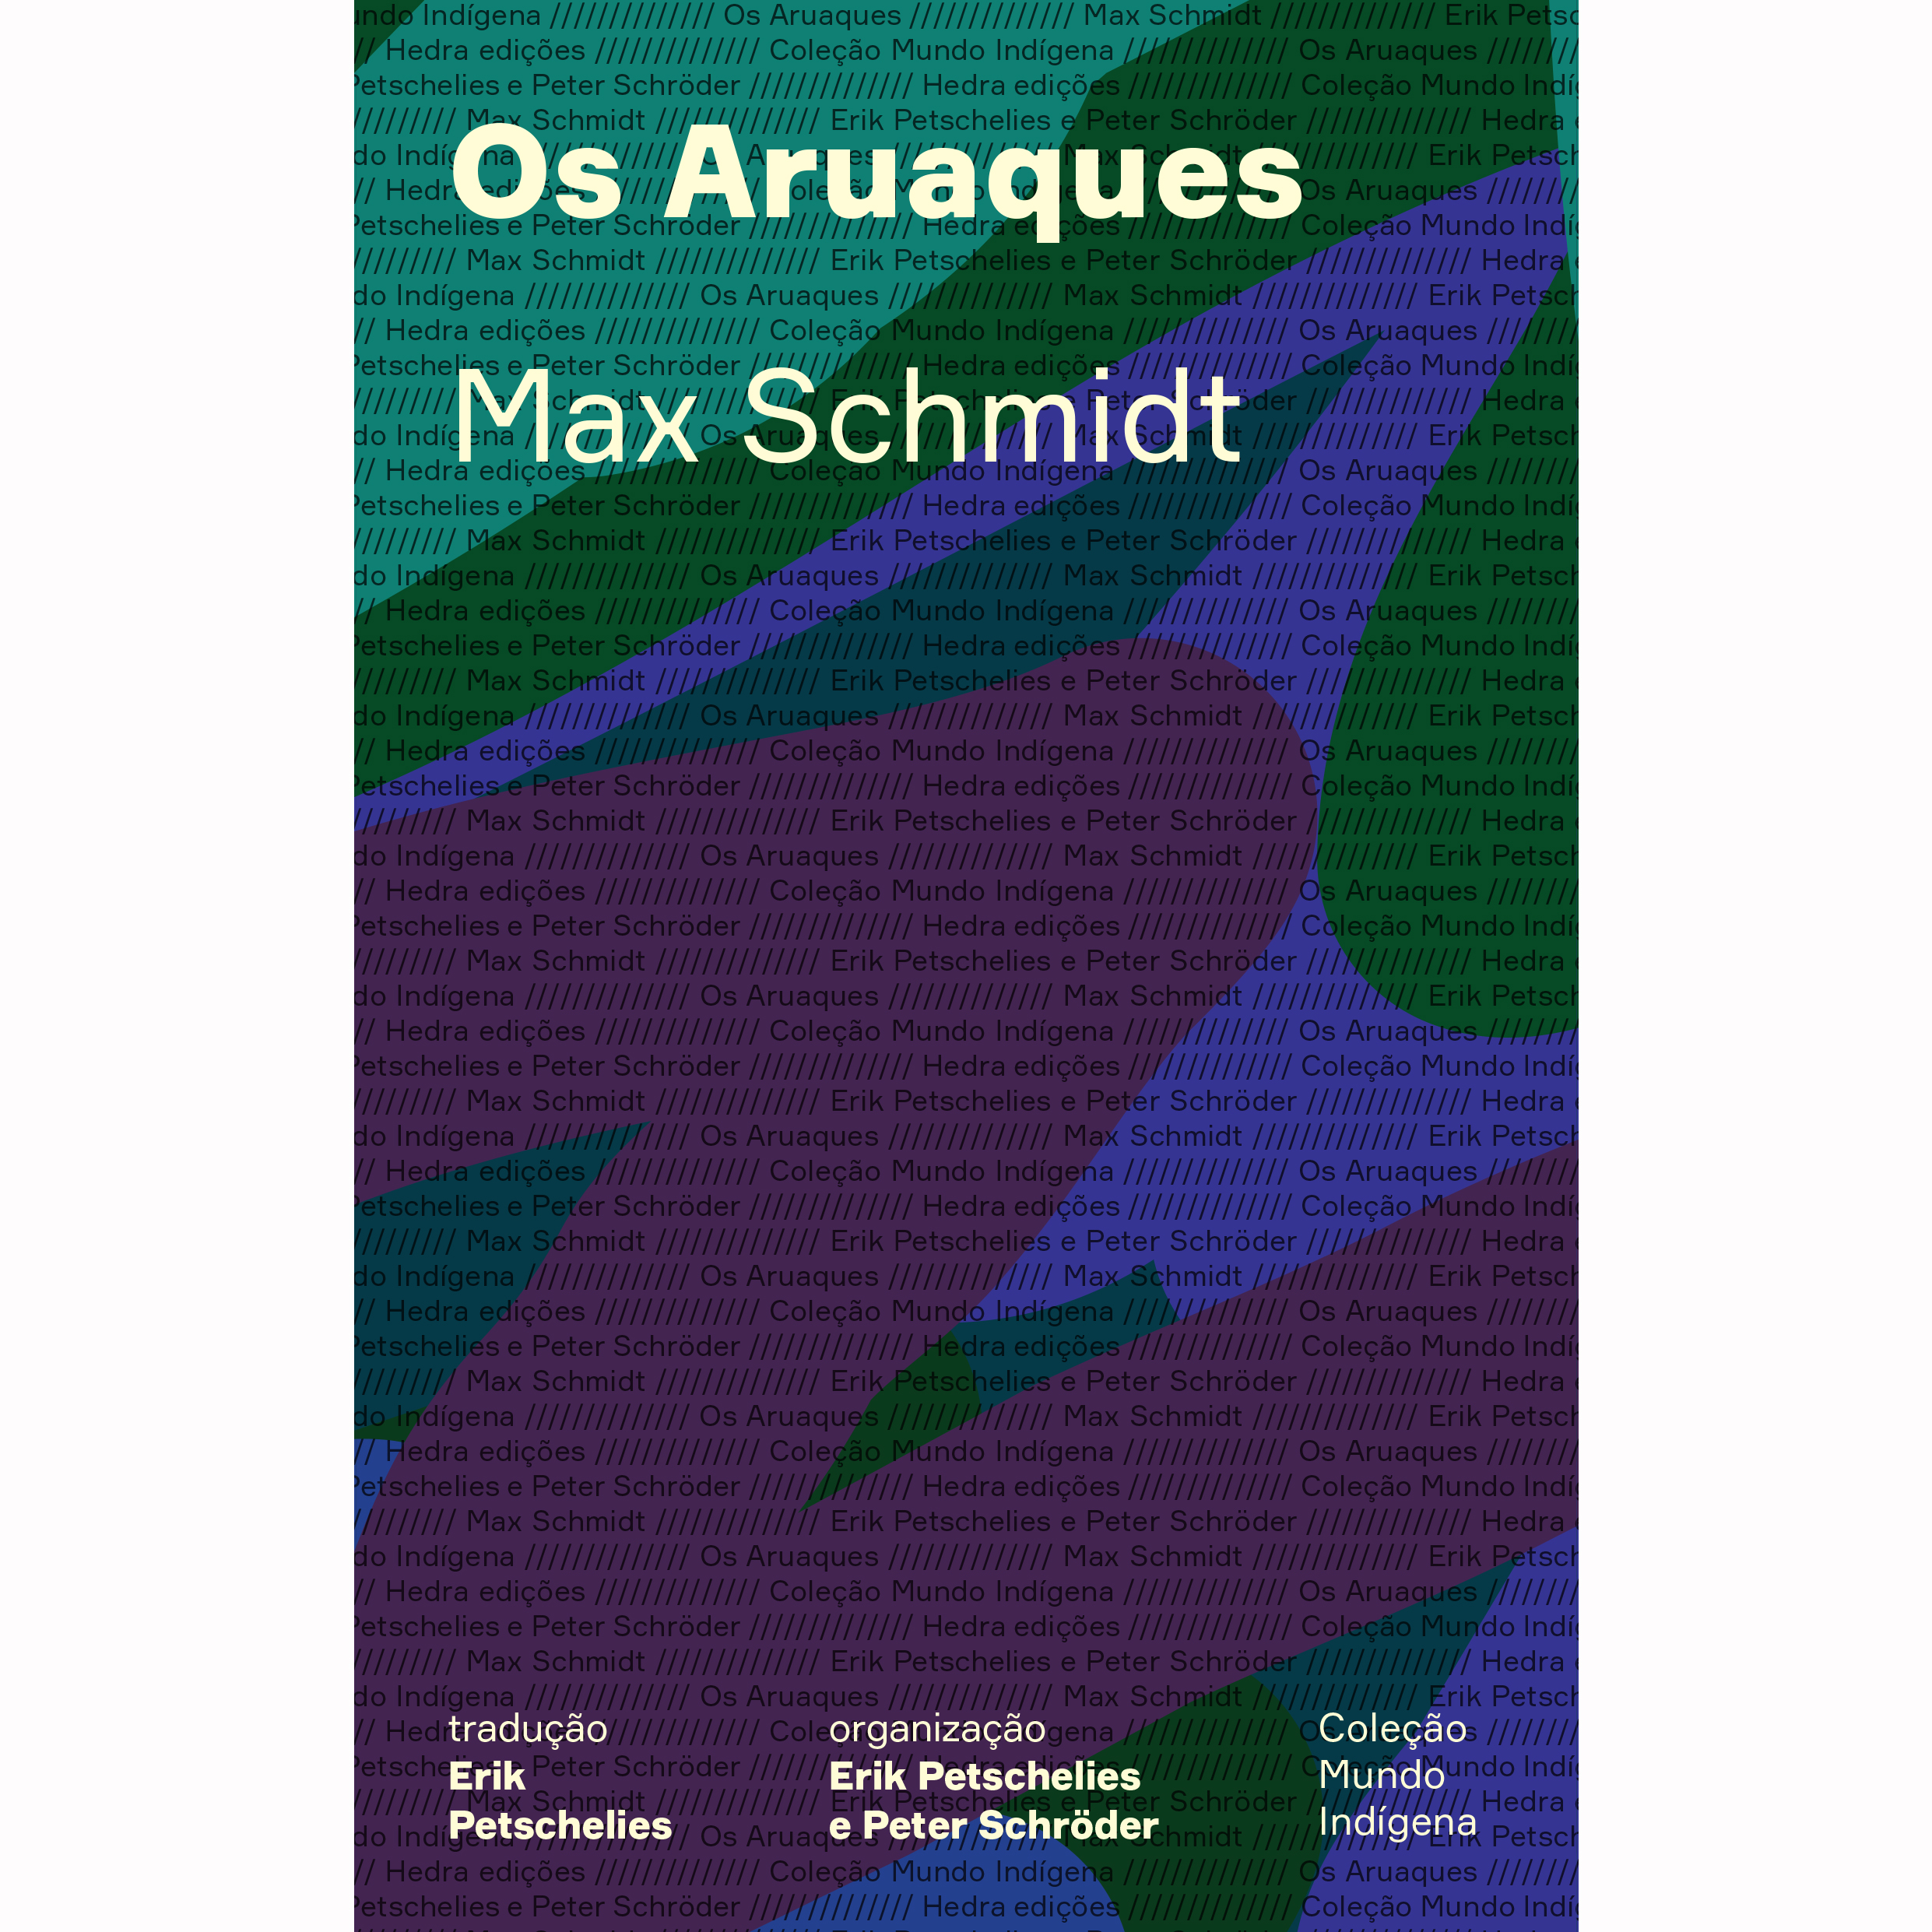
\includegraphics[width=74mm]{./CAPAS/HEDRA_ARUAQUES.jpg}
\end{center}
\hspace*{-7cm}\hrulefill\hspace*{-7cm}
\medskip

\noindent{}\textit{Os aruaques} é um \hlc{livro clássico, escrito antes da Primeira Guerra Mundial, sobre os povos indígenas falantes de línguas aruaque. Durante suas expedições, Max Schmidt já tinha observado a influência cultural dos povos aruaques sobre outros grupos, o que estimulou interesse por sua enorme expansão geográfica} nas terras baixas da América do Sul: o problema central não seria descobrir a origem geográfica dos aruaques, mas explicar sua dinâmica cultural. 

Schmidt opera com distinções claras entre língua e cultura, e conceitos como \textit{aculturação}, \textit{difusão} e \textit{mudança cultural}. Seu argumento principal é que outros autores, anteriores a ele, não teriam levantado as questões certas sobre sua expansão, por isso a falta de respostas satisfatórias. Sua teoria de fato é diferente dos antecessores, mostrando grande originalidade para a época. \textit{Die Aruaken} é a segunda tese de doutorado de Max Schmidt (1874--1950), que já tinha realizado três expedições na América do Sul, em 1900--01, 1910 e 1914.

\vfill
\noindent\begin{minipage}[c]{1\linewidth}
{\small\textbf{
\hspace*{-.1cm}Editora: Hedra\\
Título: Os Aruaques\\
Autor: Max Schmidt\\ 
ISBN: 978-65-89705-22-2\\
Páginas: 186 (provisório)\\
Formato: 13,3x21\,cm\\
Preço: R\$ 58,00\\
}}
\end{minipage}
\pagebreak

\begin{center}
\hspace*{.5cm}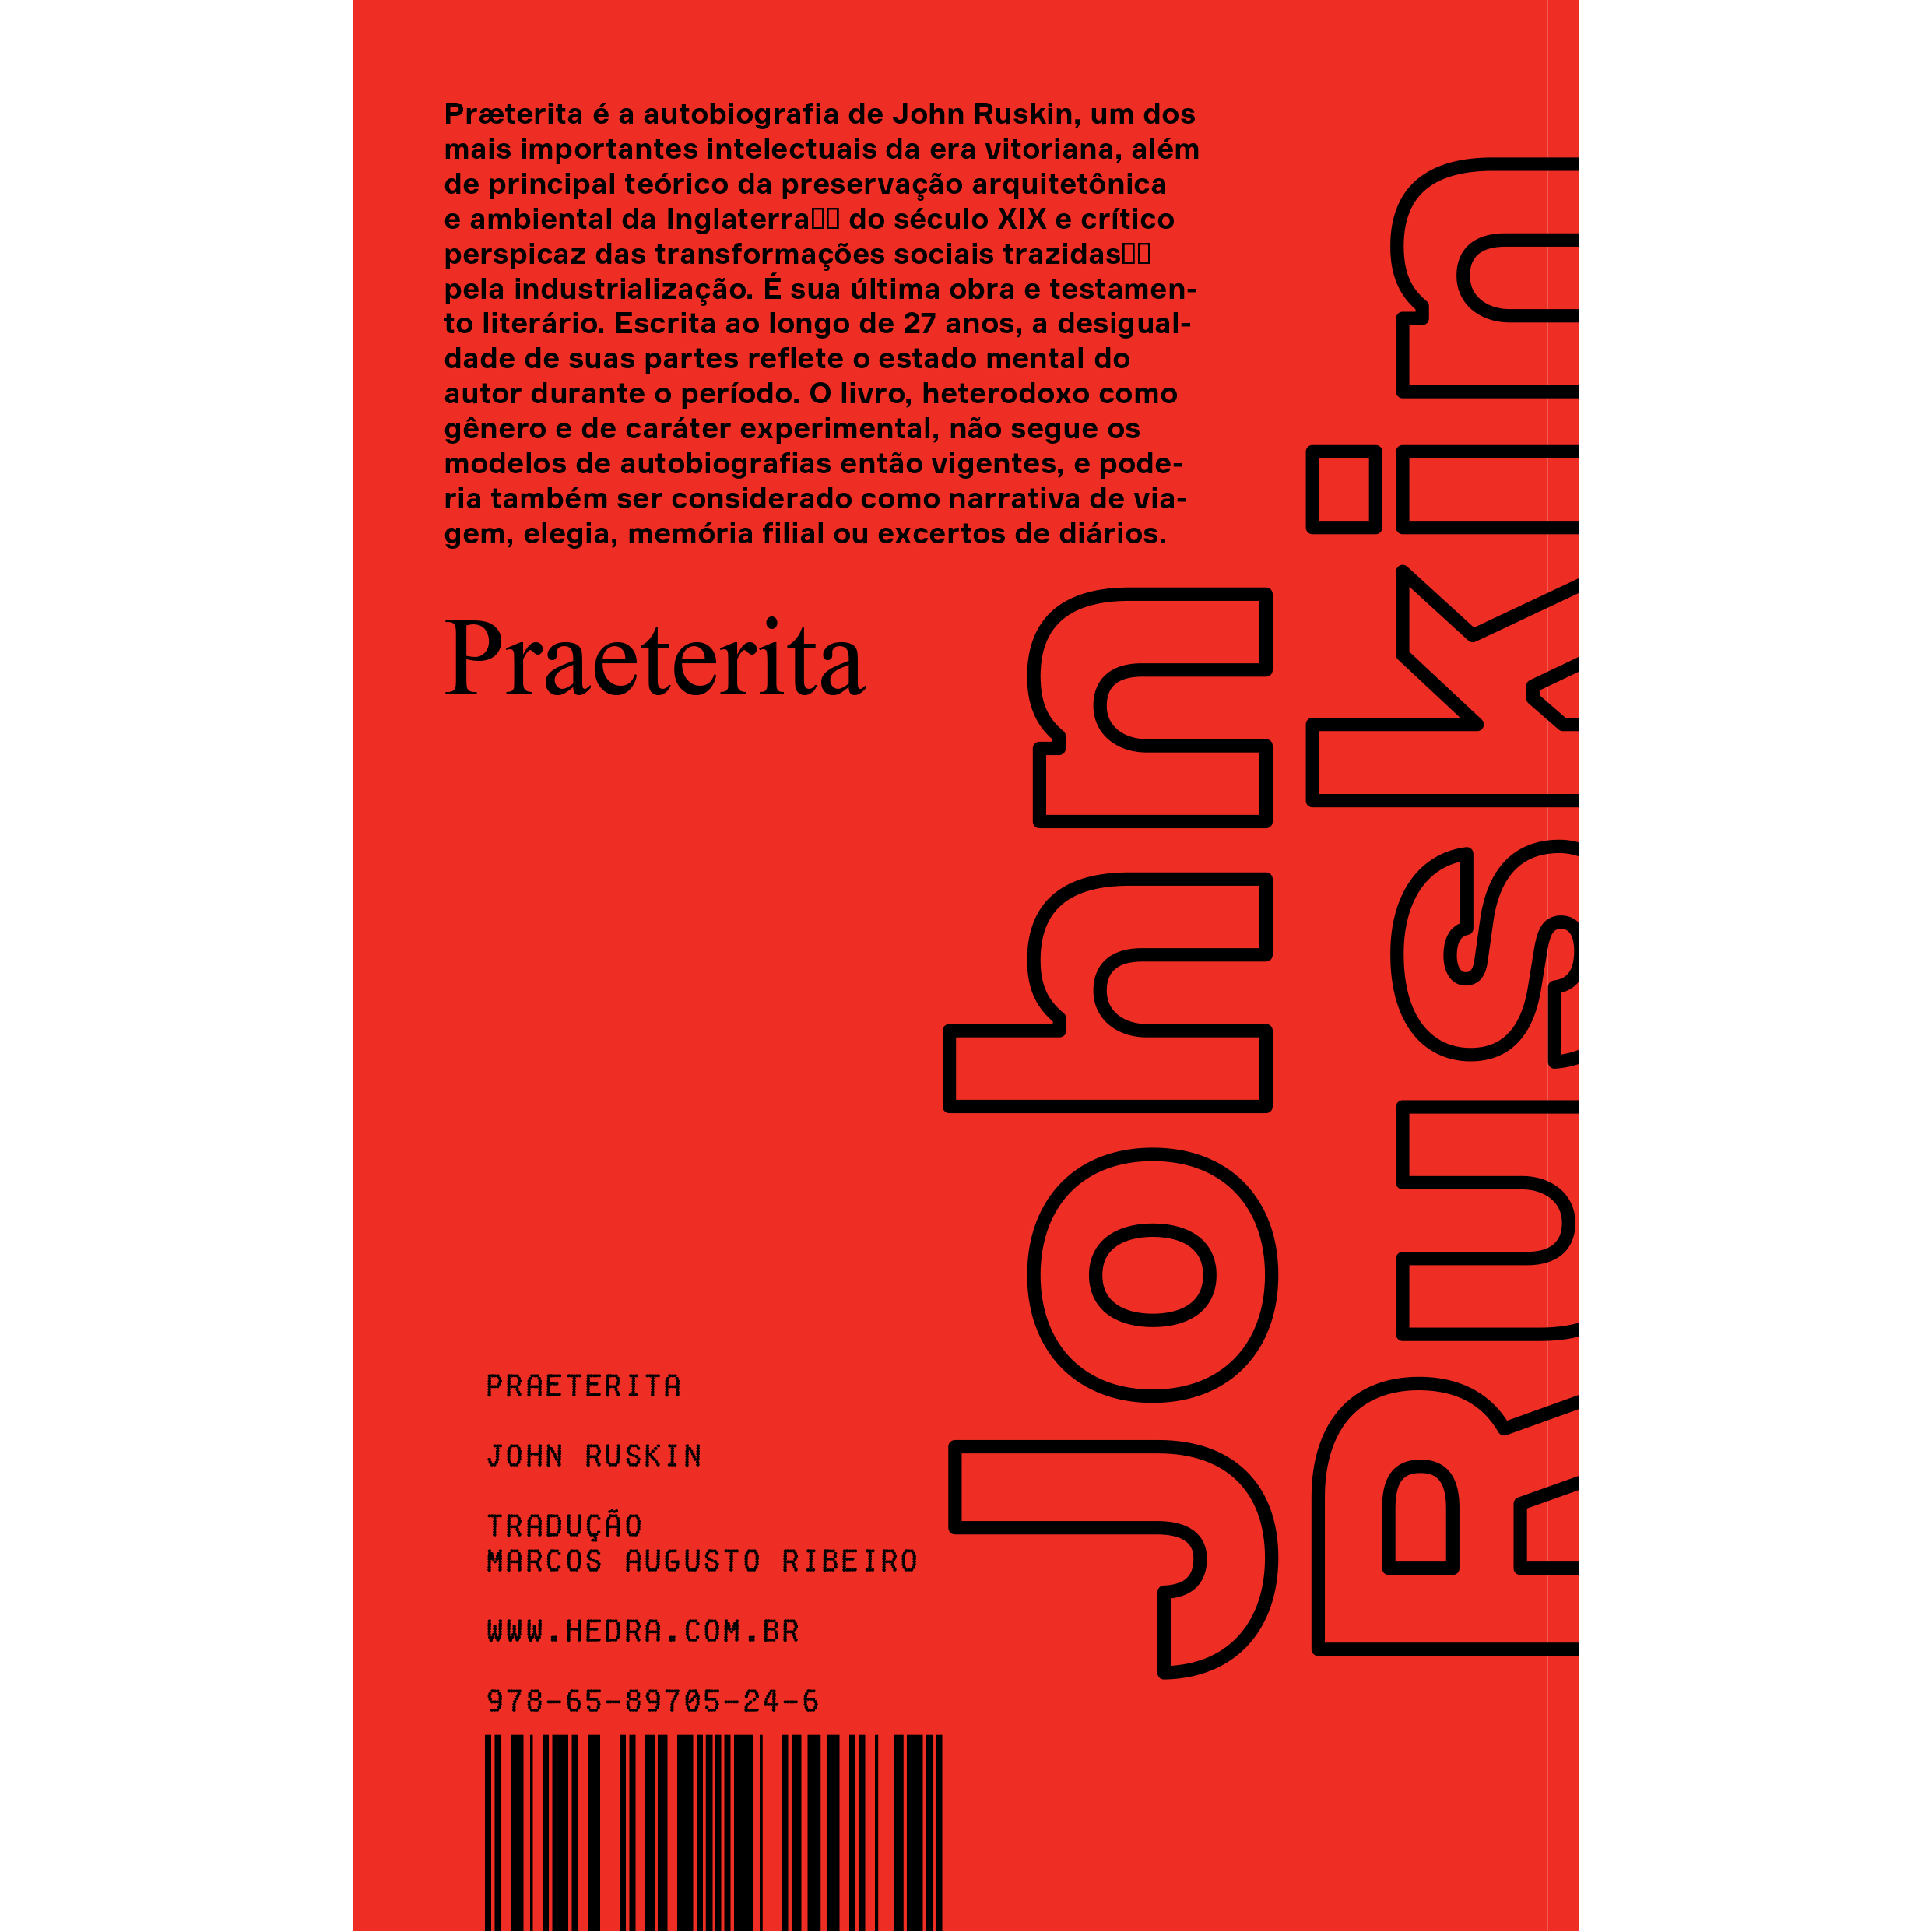
\includegraphics[width=74mm]{./CAPAS/HEDRA_RUSKIN.jpg}
\end{center}
\hspace*{-7cm}\hrulefill\hspace*{-7cm}
\medskip

\noindent{}John Ruskin (1819--1900), \hlc{foi um dos mais importantes intelectuais da era vitoriana. Principal teórico da preservação arquitetônica e ambiental da Inglaterra do século XIX e crítico perspicaz das transformações sociais trazidas ao país pela industrialização}, a qual veementemente combateu. Excêntrico, vinculado ao romantismo, grande esteta, valorizava a sensibilidade subjetiva em contraponto à razão; contraditório --- ao mesmo tempo aristocrático, reacionário e simpático ao socialismo. \textit{Praeterita}, sua autobiografia, foi sua última obra e testamento literário. Escrita ao longo de 27 anos, a desigualdade de suas partes reflete o estado mental do autor durante o período de sua elaboração. O livro, heterodoxo como gênero e de caráter ``experimental'', não segue os modelos de autobiografias então vigentes --- geralmente apresentados em termos de confissão religiosa ---, e poderia também ser considerado como narrativa de viagem, elegia, memória filial ou coleção de excertos de diários. Esta tradução contempla apenas o primeiro dos três volumes de \textit{Praeterita}.

\vfill
\noindent\begin{minipage}[c]{1\linewidth}
{\small\textbf{
\hspace*{-.1cm}Editora: Hedra\\
Título: Praeterita\\
Autor: John Ruskin\\ 
ISBN: 978-65-89705-24-6\\
Páginas: 240 (provisório)\\
Formato: 13,3x21\,cm\\
Preço: R\$ 64,90\\
}}
\end{minipage}
\pagebreak

\begin{center}
\hspace*{-3.6cm}\raisebox{5cm}{\rotatebox[origin=t]{90}{\huge\textbf{Lançamento}}}
\hspace*{3.1cm}
\includegraphics[width=74mm]{./CAPAS/HEDRA_SOCIEDADE.jpg}
\end{center}
\hspace*{-7cm}\hrulefill\hspace*{-7cm}
\medskip

\noindent{}As relações sociais passaram a figurar cada vez mais em ambientes digitais, e se transformaram em elementos de controle e disputas. É o chamado \textit{capitalismo informacional}, baseado na coleta, monitoramento e análise de dados pessoais. Se deveriam circular livremente em redes distribuídas globalmente, têm sido coletados constantemente e utilizados sem que saibamos como e por quê e, em grande parte, fora de regulamentação. \hlc{É neste cenário que as corporações têm se apropriado da tecnologia para se colocar à frente da concorrência, ao passo que governos as usam como dispositivos de controle sobre os cidadãos}. Para compreender esse fenômeno, pesquisadores se propõem a analisar neste livro as tensões da sociedade de controle, se apoiando nas contribuições de Gilbert Simondon, Félix Guattari, Gilles Deleuze, Maurizio Lazzarato, Michel Foucault, Manuel Castells, Frank Pasquale, Shoshana Zuboff, entre outros.

\vfill
\noindent\begin{minipage}[c]{1\linewidth}
{\small\textbf{
\hspace*{-.1cm}Editora: Hedra\\
Título: A sociedade de controle: manipulação e\\modulação nas redes digitais\\
Autor: Joyce Souza, Rodolfo Avelino e\\Sérgio Amadeu da Silveira (orgs.)\\ 
ISBN: 978-65-89705-19-2\\
Páginas: 160 (provisório)\\
Formato: 12,7x19,1\,cm\\
Preço: R\$ 58,00\\
}}
\end{minipage}
\pagebreak

\begin{center}
\hspace*{.5cm}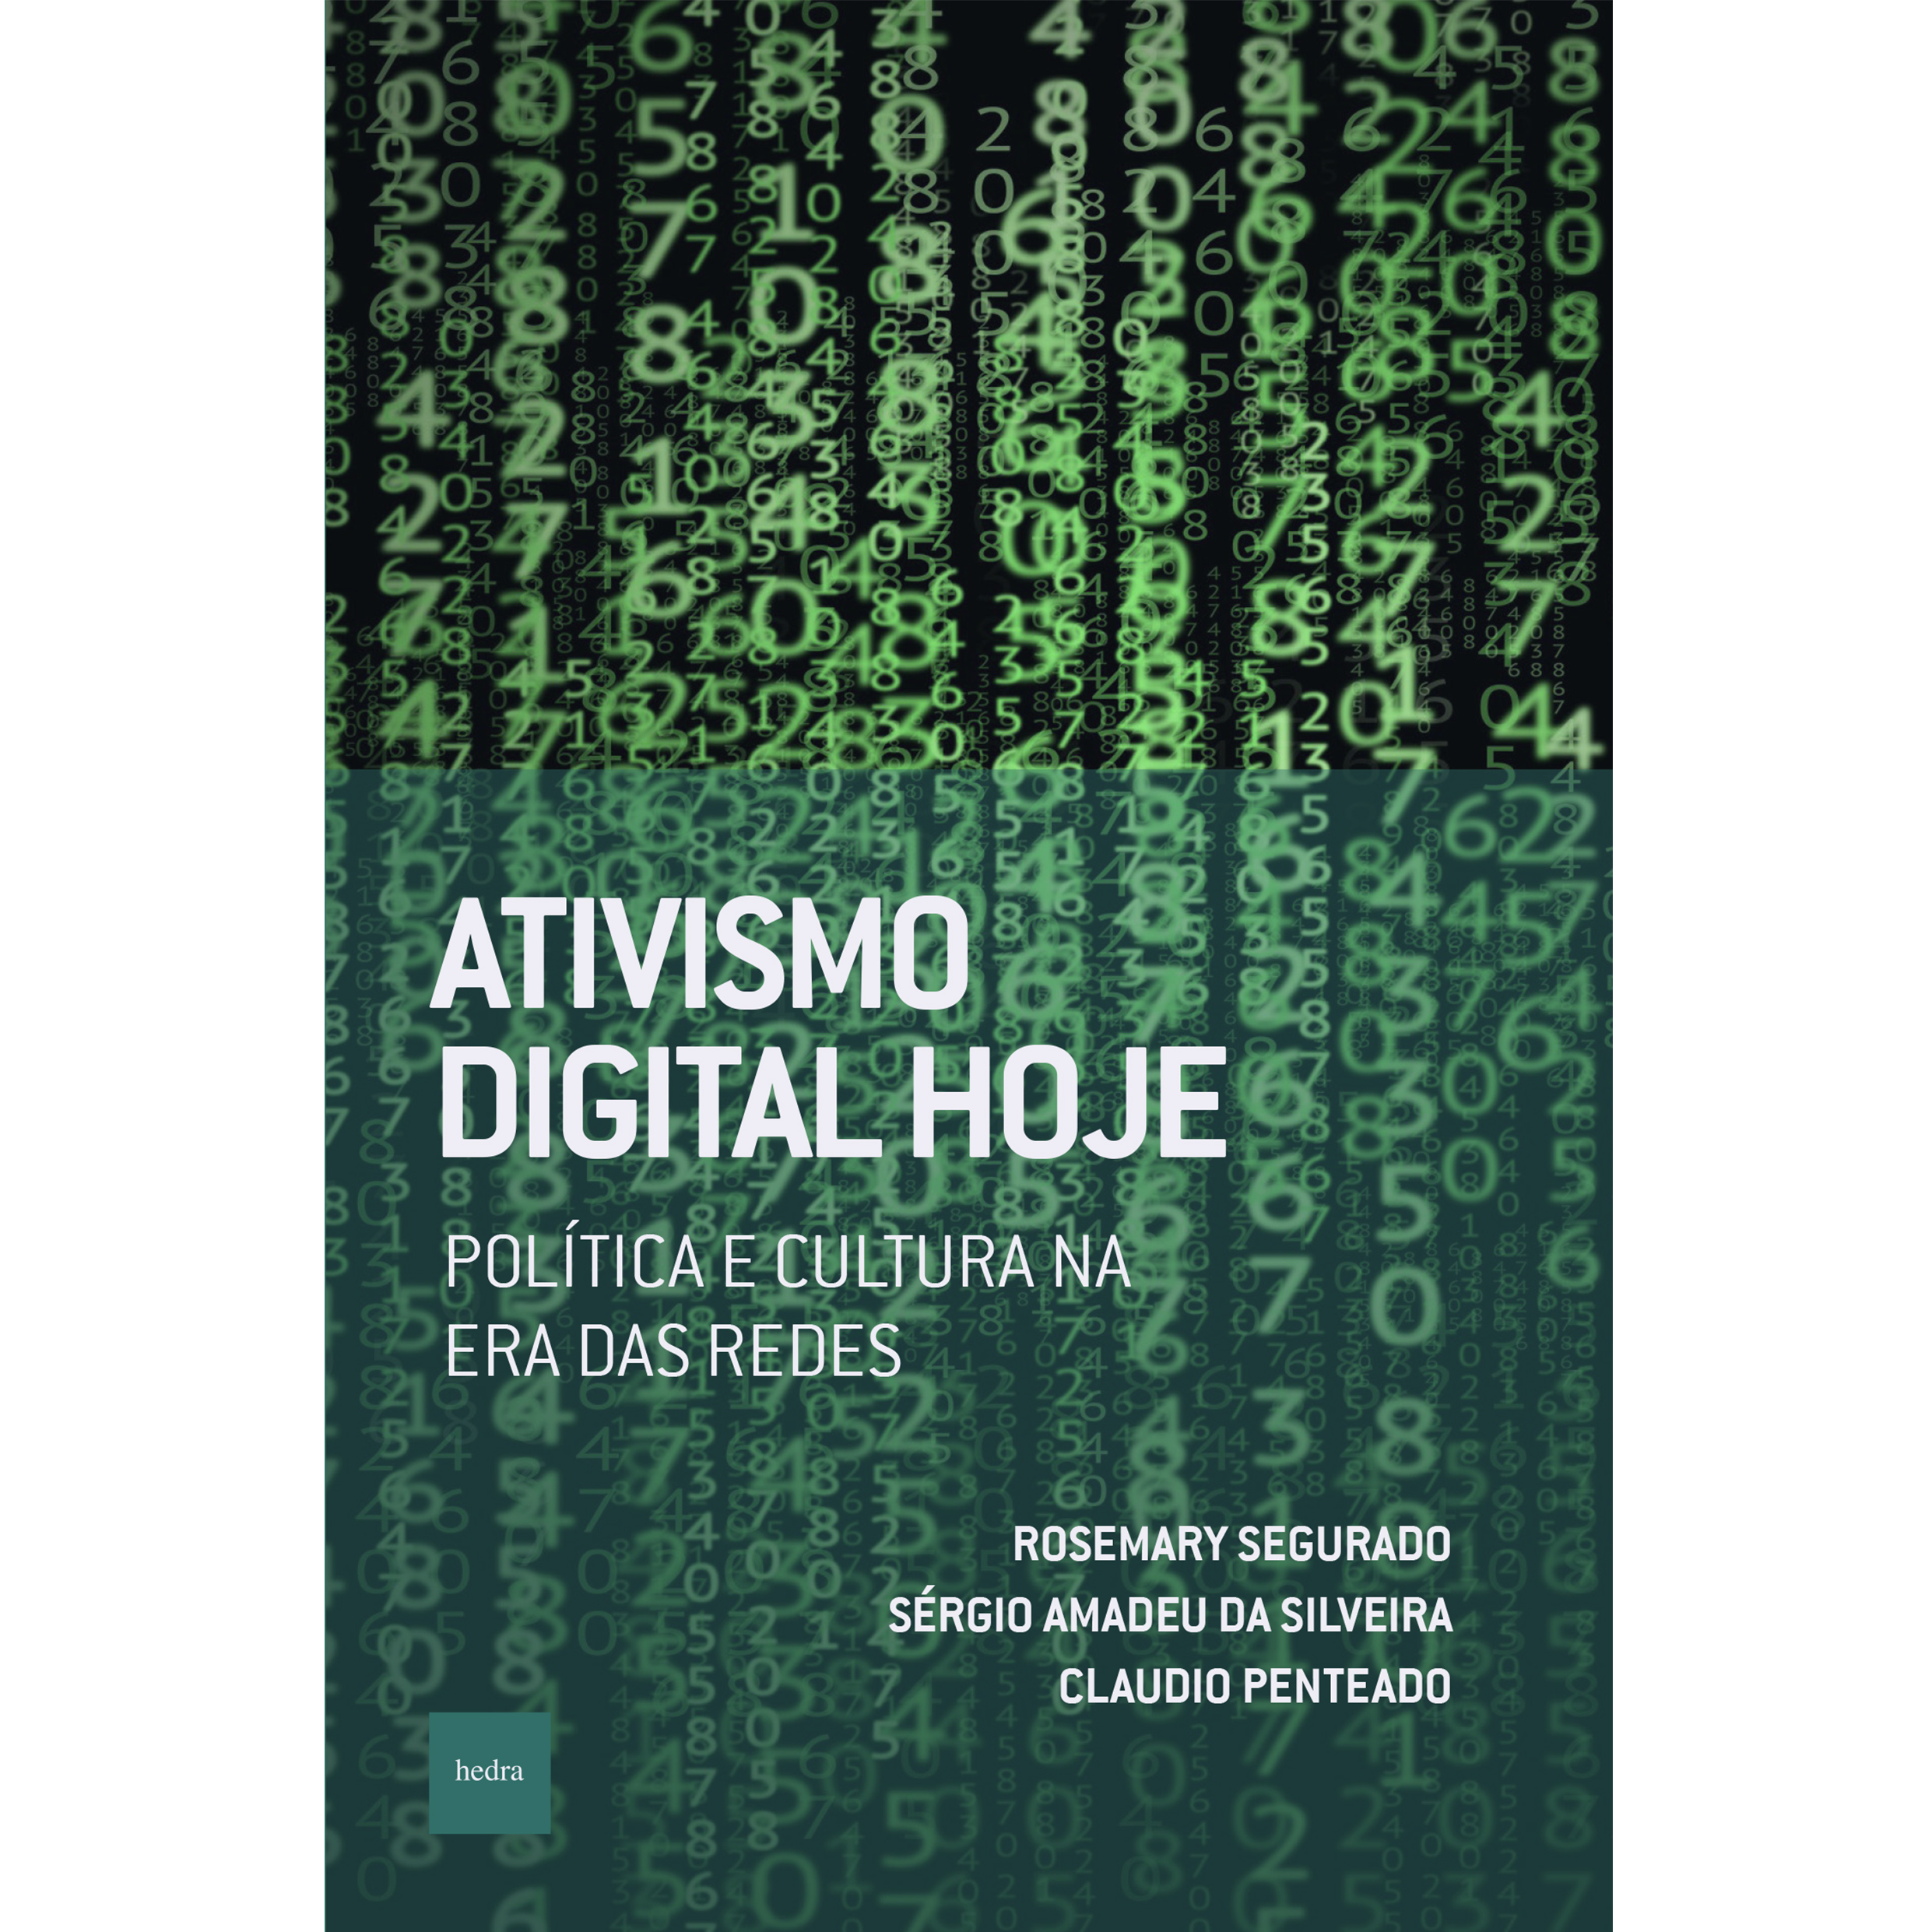
\includegraphics[width=74mm]{./CAPAS/AMADEU_ATIVISMO.jpg}
\end{center}
\hspace*{-7cm}\hrulefill\hspace*{-7cm}
\medskip

\noindent{}\textit{Ativismo digital hoje} reúne nove textos que refletem, de diferentes óticas, sobre a influência das redes sociais na política e na cultura atualmente: \hlc{ciberfeminismo, democracia digital, políticas online, ativismo online, cibervigilância, conflitos nas redes sociais, governo aberto, governança da Internet e cultura digital são alguns dos temas explorados.}
Pela abrangência do assunto, os artigos são divididos em três eixos: ciberpolítica, com enfoque na interface digital da política; ciberativismo, que percorre as alterações no campo do ativismo ocorridas desde a década de 1990; e cibercultura, que explora a emergência de práticas culturais e a expressão de subjetividades em consonância com as novas práticas comunicacionais do meio digital.

\vfill
\noindent\begin{minipage}[c]{1\linewidth}
{\small\textbf{
\hspace*{-.1cm}Editora: Hedra\\
Título: Ativismo digital hoje: política e\\cultura na era das redes\\
Autor: Rosemary Segurado, Claudio Penteado e\\Sérgio Amadeu da Silveira (orgs.)\\ 
ISBN: 978-85-7715-616-0\\
Páginas: 220 (provisório)\\
Formato: 12,7x19,1\,cm\\
Preço: R\$ 72,00\\
}}
\end{minipage}
\pagebreak

\begin{center}
\hspace*{-3.6cm}\raisebox{5cm}{\rotatebox[origin=t]{90}{\huge\textbf{Lançamento}}}
\hspace*{3.1cm}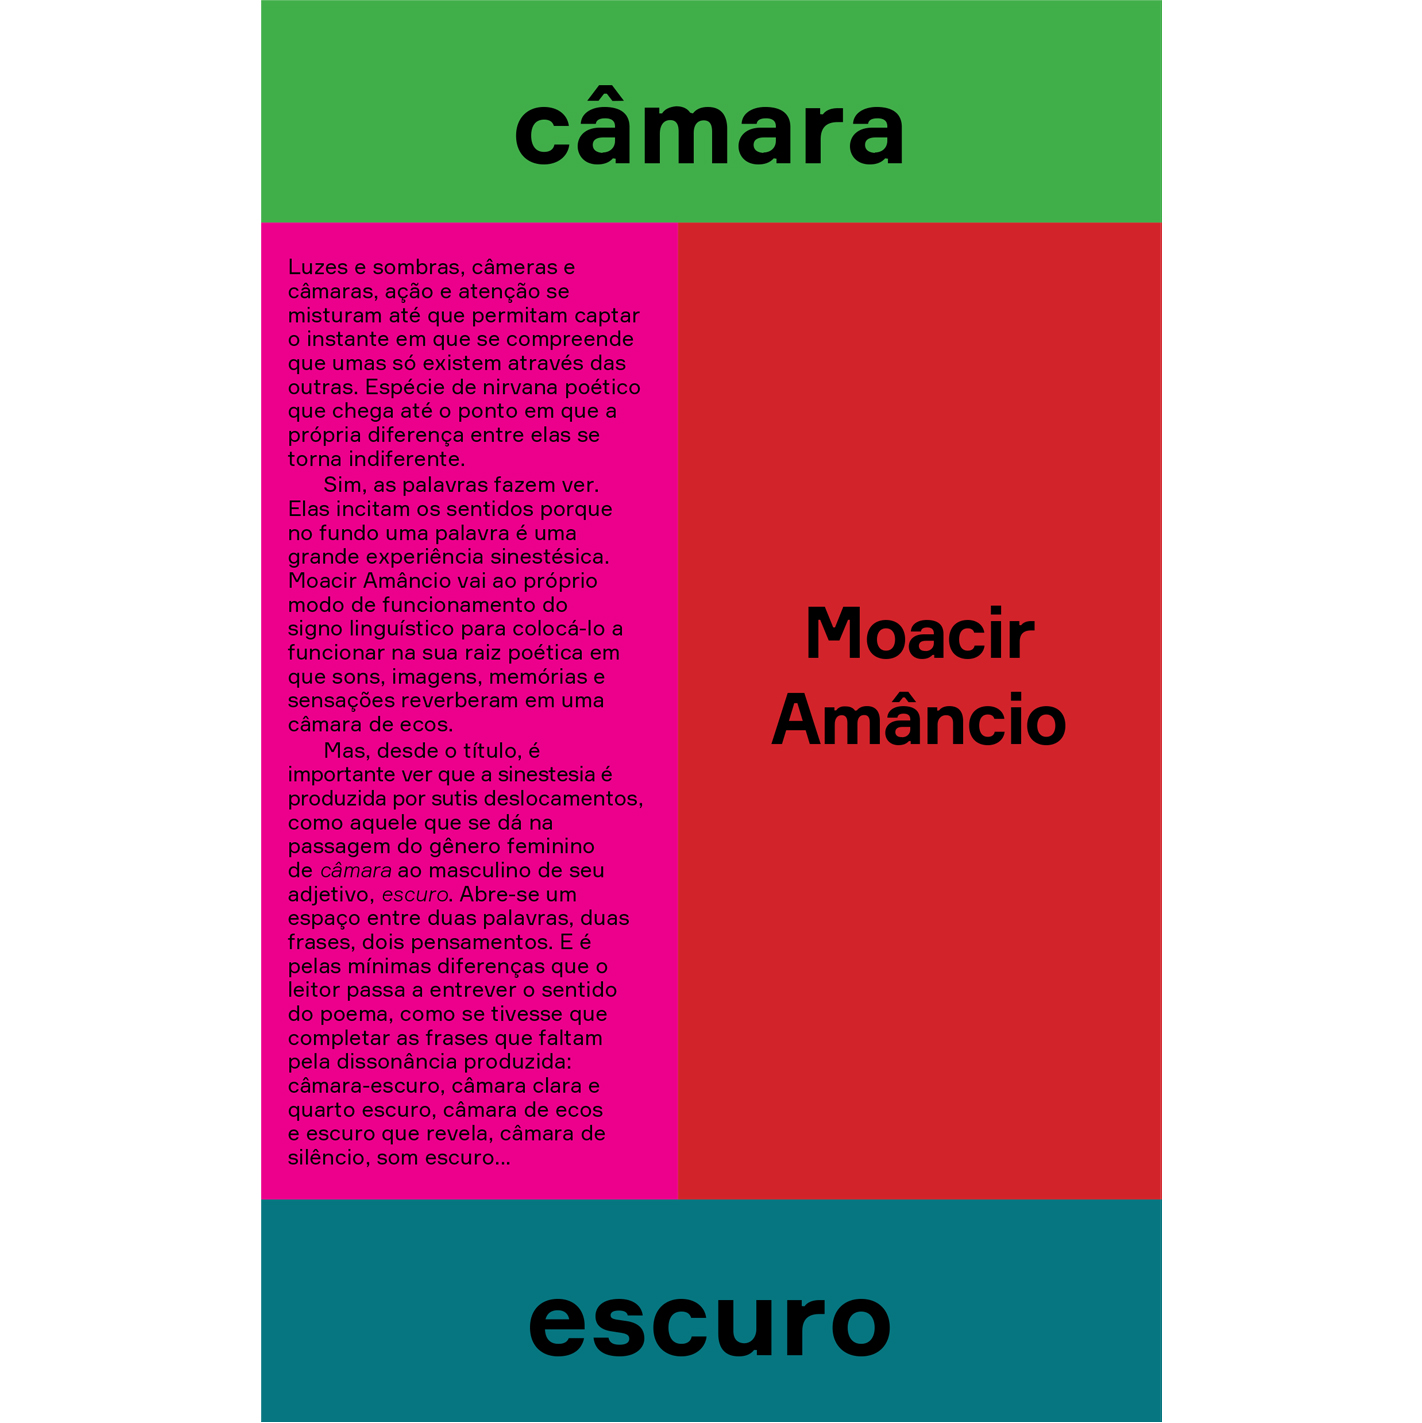
\includegraphics[width=74mm]{./CAPAS/HEDRA_CAMARA.jpg}
\end{center}
\hspace*{-7cm}\hrulefill\hspace*{-7cm}
\medskip

\noindent{}Inserir.

\vfill
\noindent\begin{minipage}[c]{1\linewidth}
{\small\textbf{
\hspace*{-.1cm}Editora: Hedra\\
Título: Câmara escuro\\
Autor: Moacir Amâncio\\ 
ISBN: 978-65-89705-27-7\\
Páginas: 73 (provisório)\\
Formato: 13,3x21\,cm\\
Preço: R\$ 34,00\\
}}
\end{minipage}
\pagebreak

\begin{center}
\hspace*{.5cm}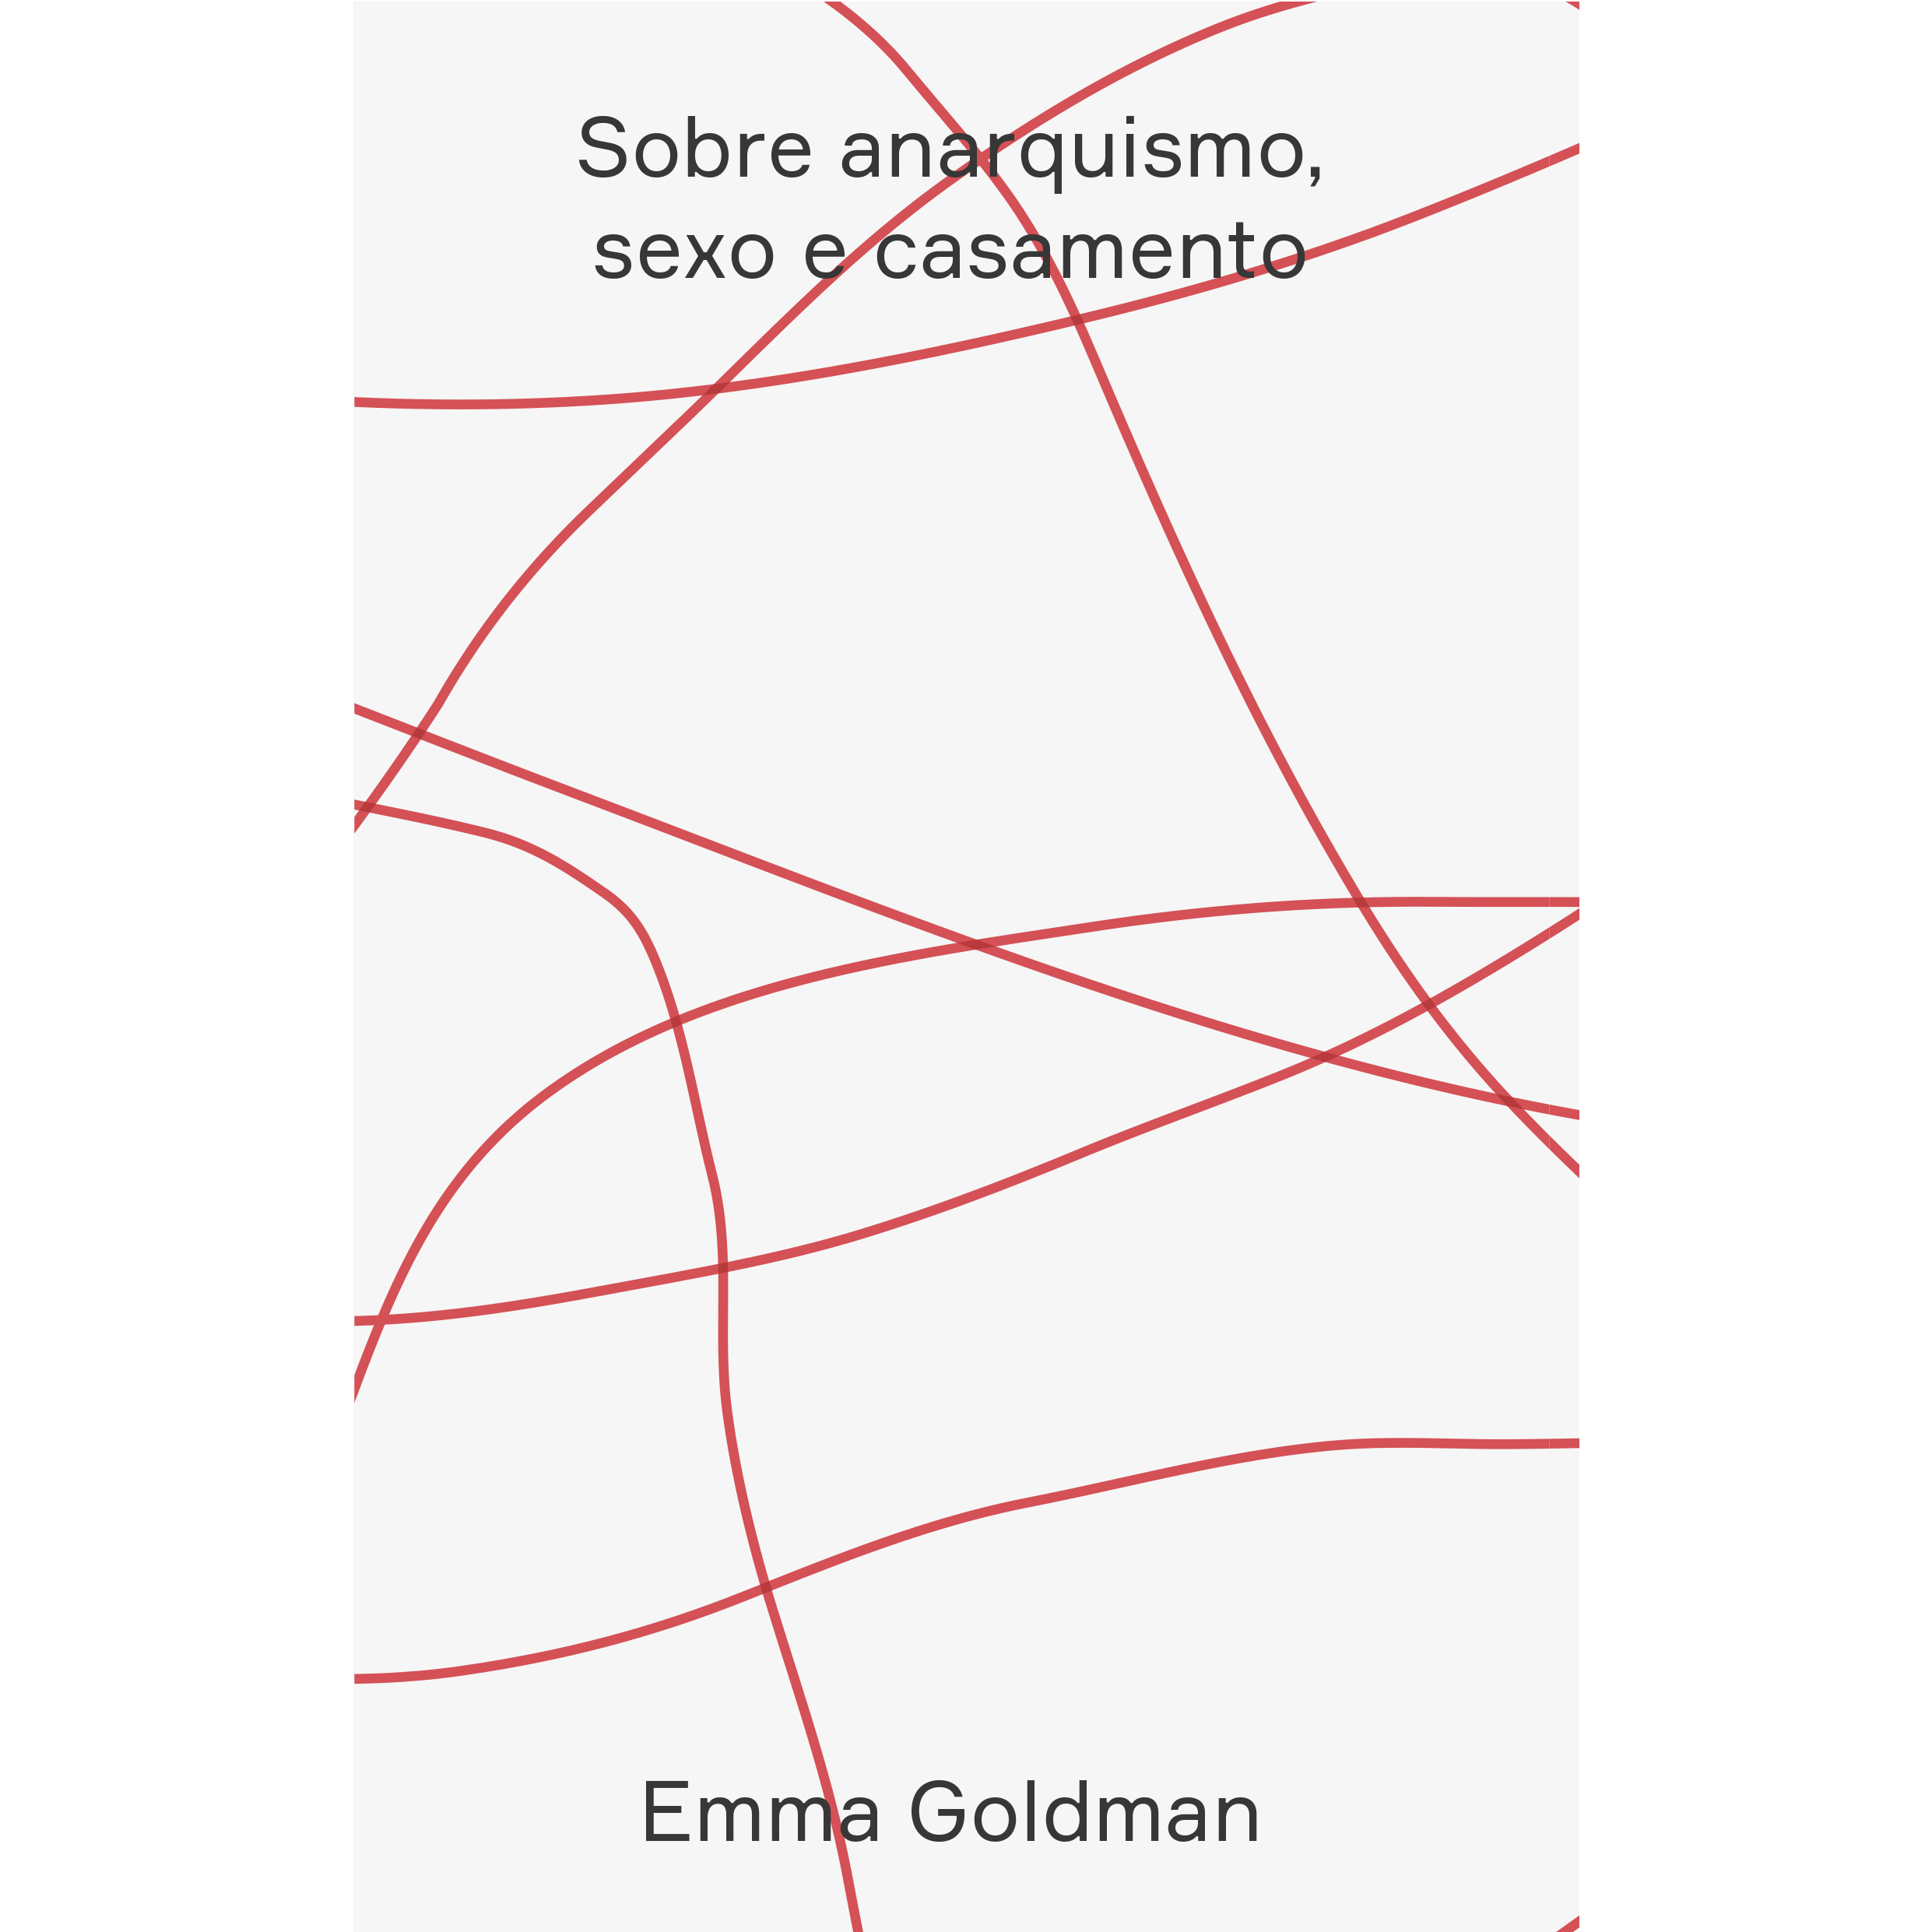
\includegraphics[width=74mm]{./CAPAS/HEDRA_GOLDMAN.jpg}
\end{center}
\hspace*{-7cm}\hrulefill\hspace*{-7cm}
\medskip

\noindent{}Sob perspectiva da implacável anarquista que foi Emma Goldman, \textit{Sobre anarquismo, sexo e casamento} trata de temas como o \hlc{controle de natalidade, o puritanismo norte-americano, a repressão sexual, o amor livre, o ciúme, a prostituição, a homossexualidade, a desigualdade entre os sexos, a maternidade, a emancipação feminina, o movimento sufragista na Inglaterra e Estados Unidos e a trajetória de uma série de mulheres extraordinárias}, dentre elas heroínas e mártires do movimento revolucionário russo. 

O contexto no qual esses textos foram escritos passou pela Primeira Guerra Mundial, a Revolução Russa e a ascensão do fascismo italiano e do nacional-socialismo na Alemanha. Dada a sua condição de russa, judia, anarquista e crítica implacável do puritanismo estadunidense à autocracia soviética, tornavam-lhe ainda mais vulnerável --- dos Estados Unidos à Rússia, e nos mais diferentes círculos.

\vfill
\noindent\begin{minipage}[c]{.5\linewidth}
{\small\textbf{
\hspace*{-.1cm}Editora: Hedra\\
Título: Sobre anarquismo,\\sexo e casamento\\
Autor: Emma Goldman\\ 
ISBN: 978-65-89705-23-9\\
Páginas: 264 (provisório)\\
Formato: 13,3x21\,cm\\
Preço: R\$ 69,90\\
}}
\end{minipage}
\pagebreak

\begin{center}
\hspace*{-3.6cm}\raisebox{5cm}{\rotatebox[origin=t]{90}{\huge\textbf{Lançamento}}}
\hspace*{3.1cm}
\includegraphics[width=74mm]{./CAPAS/BREVE.jpg}
\end{center}
\hspace*{-7cm}\hrulefill\hspace*{-7cm}
\medskip

\noindent{}As plataformas digitais foram fundamentais para diminuir o impacto do distanciamento social durante a pandemia da Covid-19. A internet e as redes sociais digitais passaram a ser a janela para o mundo para muitos e através dela eram realizadas atividades profissionais, encontros entre amigos e familiares, compras e vendas online, aulas, consultas médicas e acesso à cultura. 

\hlc{A vida estava, enfim, circunscrita às telas de nossos computadores e celulares, embora a maior parte da população brasileira não pudesse se manter em isolamento social. Mas foi também por meio delas verificamos o aumento do compartilhamento de informações falsas}, mentiras e boatos sobre a pandemia. O Brasil ocupou o triste lugar de país que mais compartilha informações falsas ou duvidosas sobre o coronavírus.

\vfill
\noindent\begin{minipage}[c]{1\linewidth}
{\small\textbf{
\hspace*{-.1cm}Editora: Hedra\\
Título: Democracia e desinformação: fake news na internet\\
Autor: Rosemary Segurado (org.)\\ 
ISBN: 978-65-89705-34-5\\
Páginas: Inserir.\\
Formato: 12,7x19,1\,cm\\
Preço: R\$ Inserir.\\
}}
\end{minipage}
\pagebreak

\begin{center}
\hspace*{.5cm}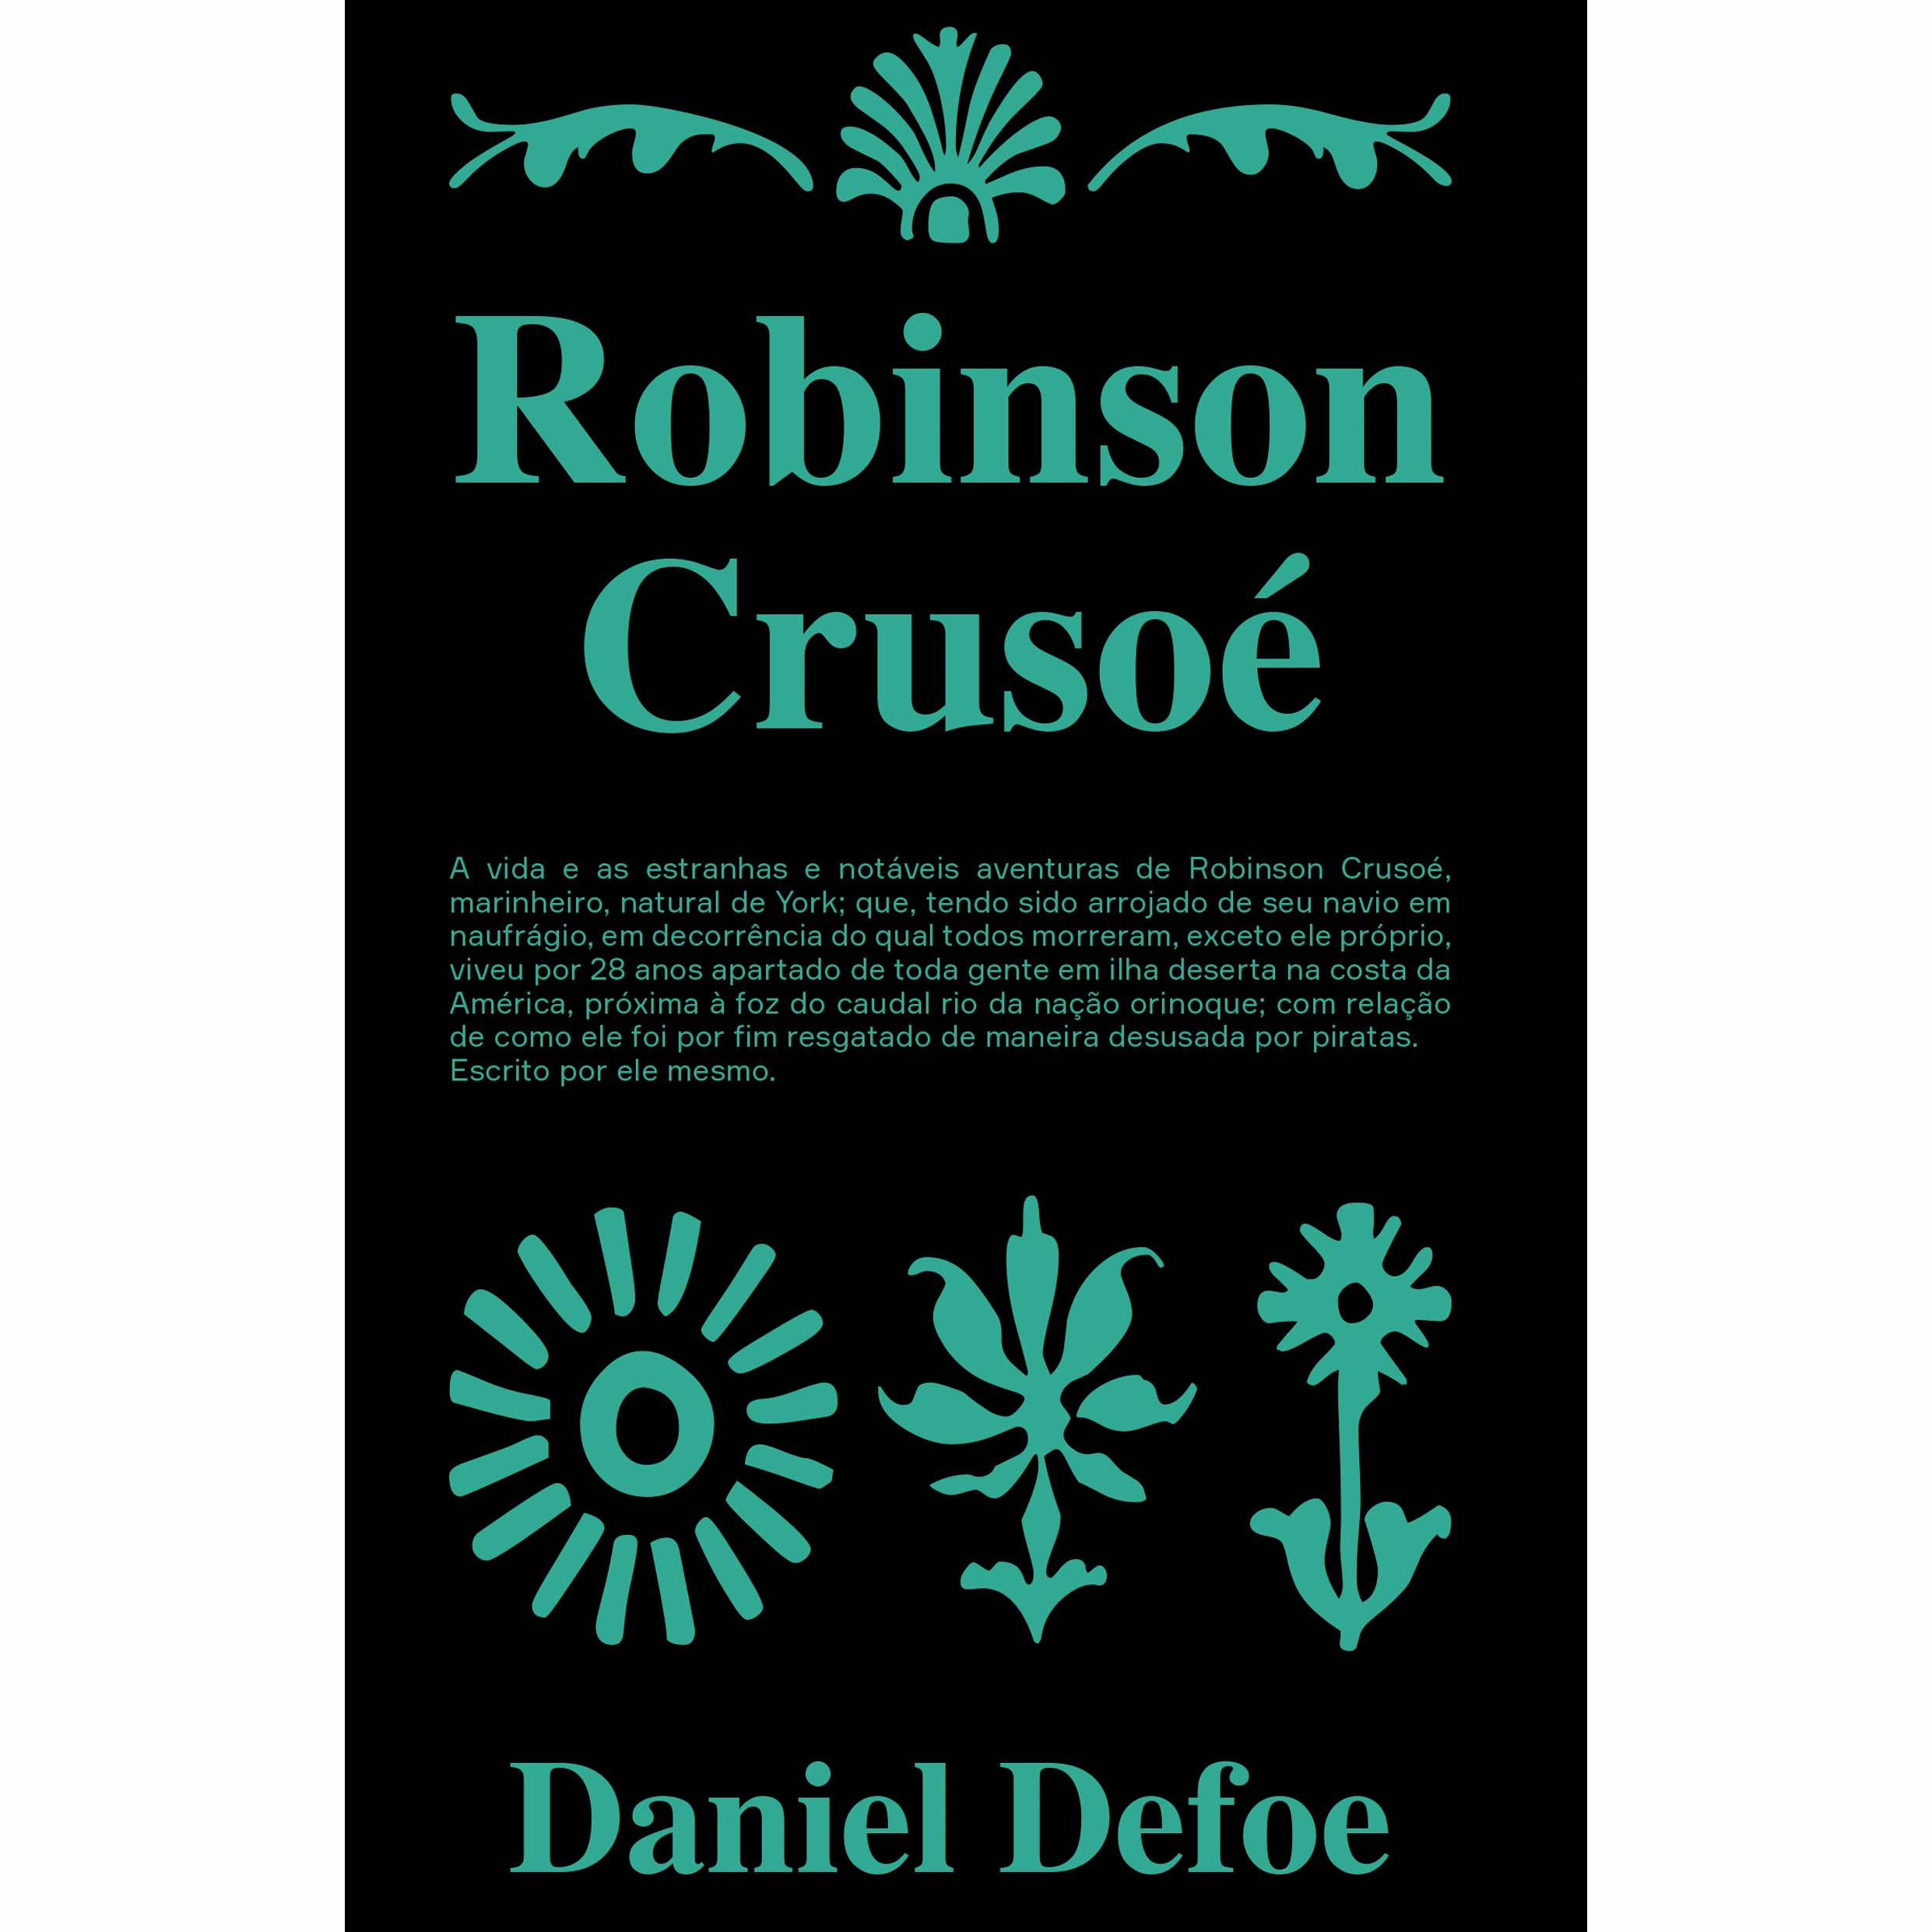
\includegraphics[width=74mm]{./CAPAS/HEDRA_ROBINSON.jpg}
\end{center}
\hspace*{-7cm}\hrulefill\hspace*{-7cm}
\medskip

\noindent{}Daniel Defoe (1660--1731) escreveu \textit{Robinson Crusoé} em primeira pessoa, livro que segue o modo epistolar de um diário. Publicado durante uma época conhecida por fazer ascender o romance, seus detalhes objetivos influenciaram Herman Melville, em \textit{Moby Dick} (1851).

O náufrago Robinson Crusoé, que dá nome ao livro, \hlc{é uma espécie de autobiografia fictícia de um homem que passou 28 anos em uma remota ilha tropical encontrando canibais cativos e revoltosos antes de ser resgatado}. Originalmente publicado na forma de folhetins no The Daily Post, é um clássico lido em diversas versões --- até mesmo em adaptações infanto-juvenis. É, todavia, uma obra complexa e seus contornos históricos até hoje propõem discussões. 

\vfill
\noindent\begin{minipage}[c]{1\linewidth}
{\small\textbf{
\hspace*{-.1cm}Editora: Hedra\\
Título: Robinson Crusoé\\
Autor: Daniel Defoe\\ 
ISBN: 978-65-89705-31-4\\
Páginas: 350 (provisório)\\
Formato: 13,3x21\,cm\\
Preço: R\$ 89,00\\
}}
\end{minipage}
\pagebreak

\begin{center}
\hspace*{-3.6cm}\raisebox{5cm}{\rotatebox[origin=t]{90}{\huge\textbf{Lançamento}}}
\hspace*{3.1cm}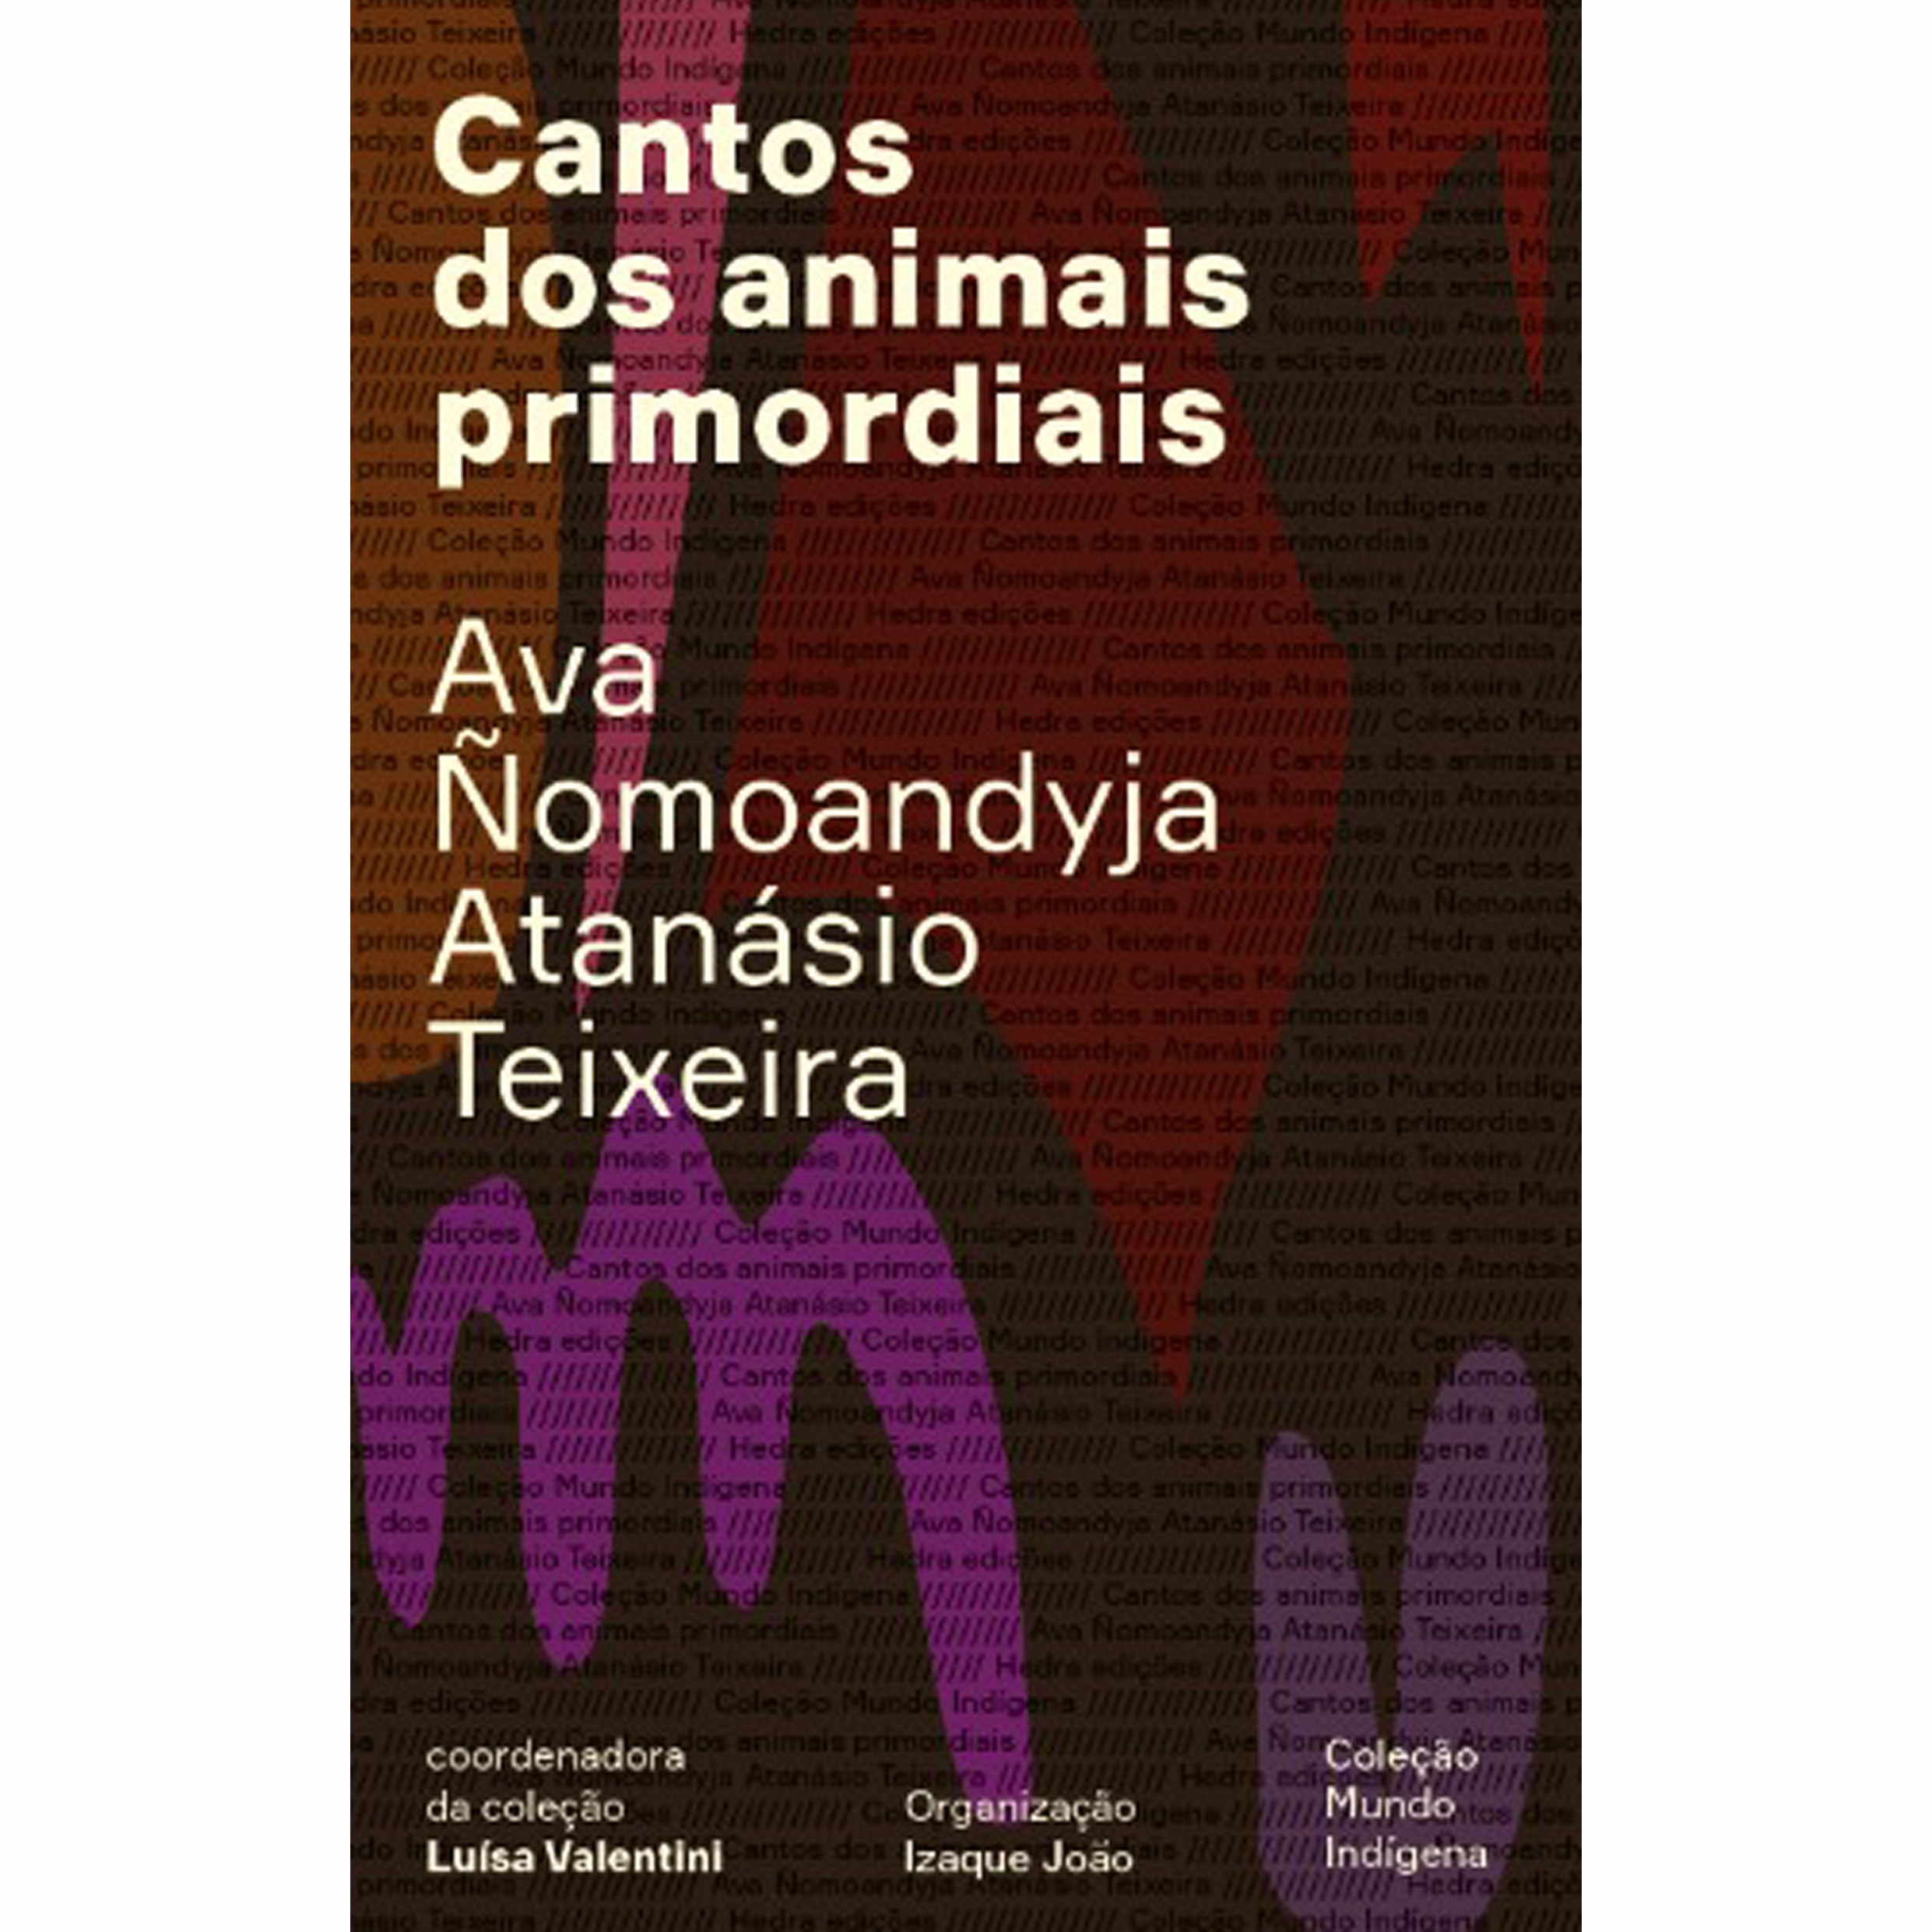
\includegraphics[width=74mm]{./CAPAS/HEDRA_CANTOS.jpg}
\end{center}
\hspace*{-7cm}\hrulefill\hspace*{-7cm}
\medskip

\noindent{}Neste livro são apresentadas \hlc{26 histórias de aves e outros animais da mata, acompanhados pelos cantos \textit{guahu} que cantam sua história desde o princípio dos tempos.} Esses \textit{guahu} fazem parte de um conjunto maior de cantos, rezas e danças dominados por Atanásio Teixeira ou Ava Ñomoandyja, um dos mais prestigiosos xamãs do povo Guarani Kaiowá. As narrativas e explicações que acompanham os cantos foram elaboradas pelo historiador Izaque João, a partir de falas e orientações de Atanásio Teixeira ao longo dos últimos seis anos. 

Os processos de seleção, transcrição e tradução para esta edição bilíngue também foram feitos em diálogo com o xamã e as versões em português dos textos e cantos \textit{guahu} são um exercício de aproximação de suas belas palavras.

\vfill
\noindent\begin{minipage}[c]{1\linewidth}
{\small\textbf{
\hspace*{-.1cm}Editora: Hedra\\
Título: Cantos dos animais primordiais\\
Autor: Ava Ñomoandyja Atanásio Teixeira\\ 
ISBN: 978-65-89705-30-7\\
Páginas: Inserir.\\
Formato: 13,3x21\,cm\\
Preço: R\$ Inserir.\\
}}
\end{minipage}
\pagebreak

\begin{center}
\hspace*{.5cm}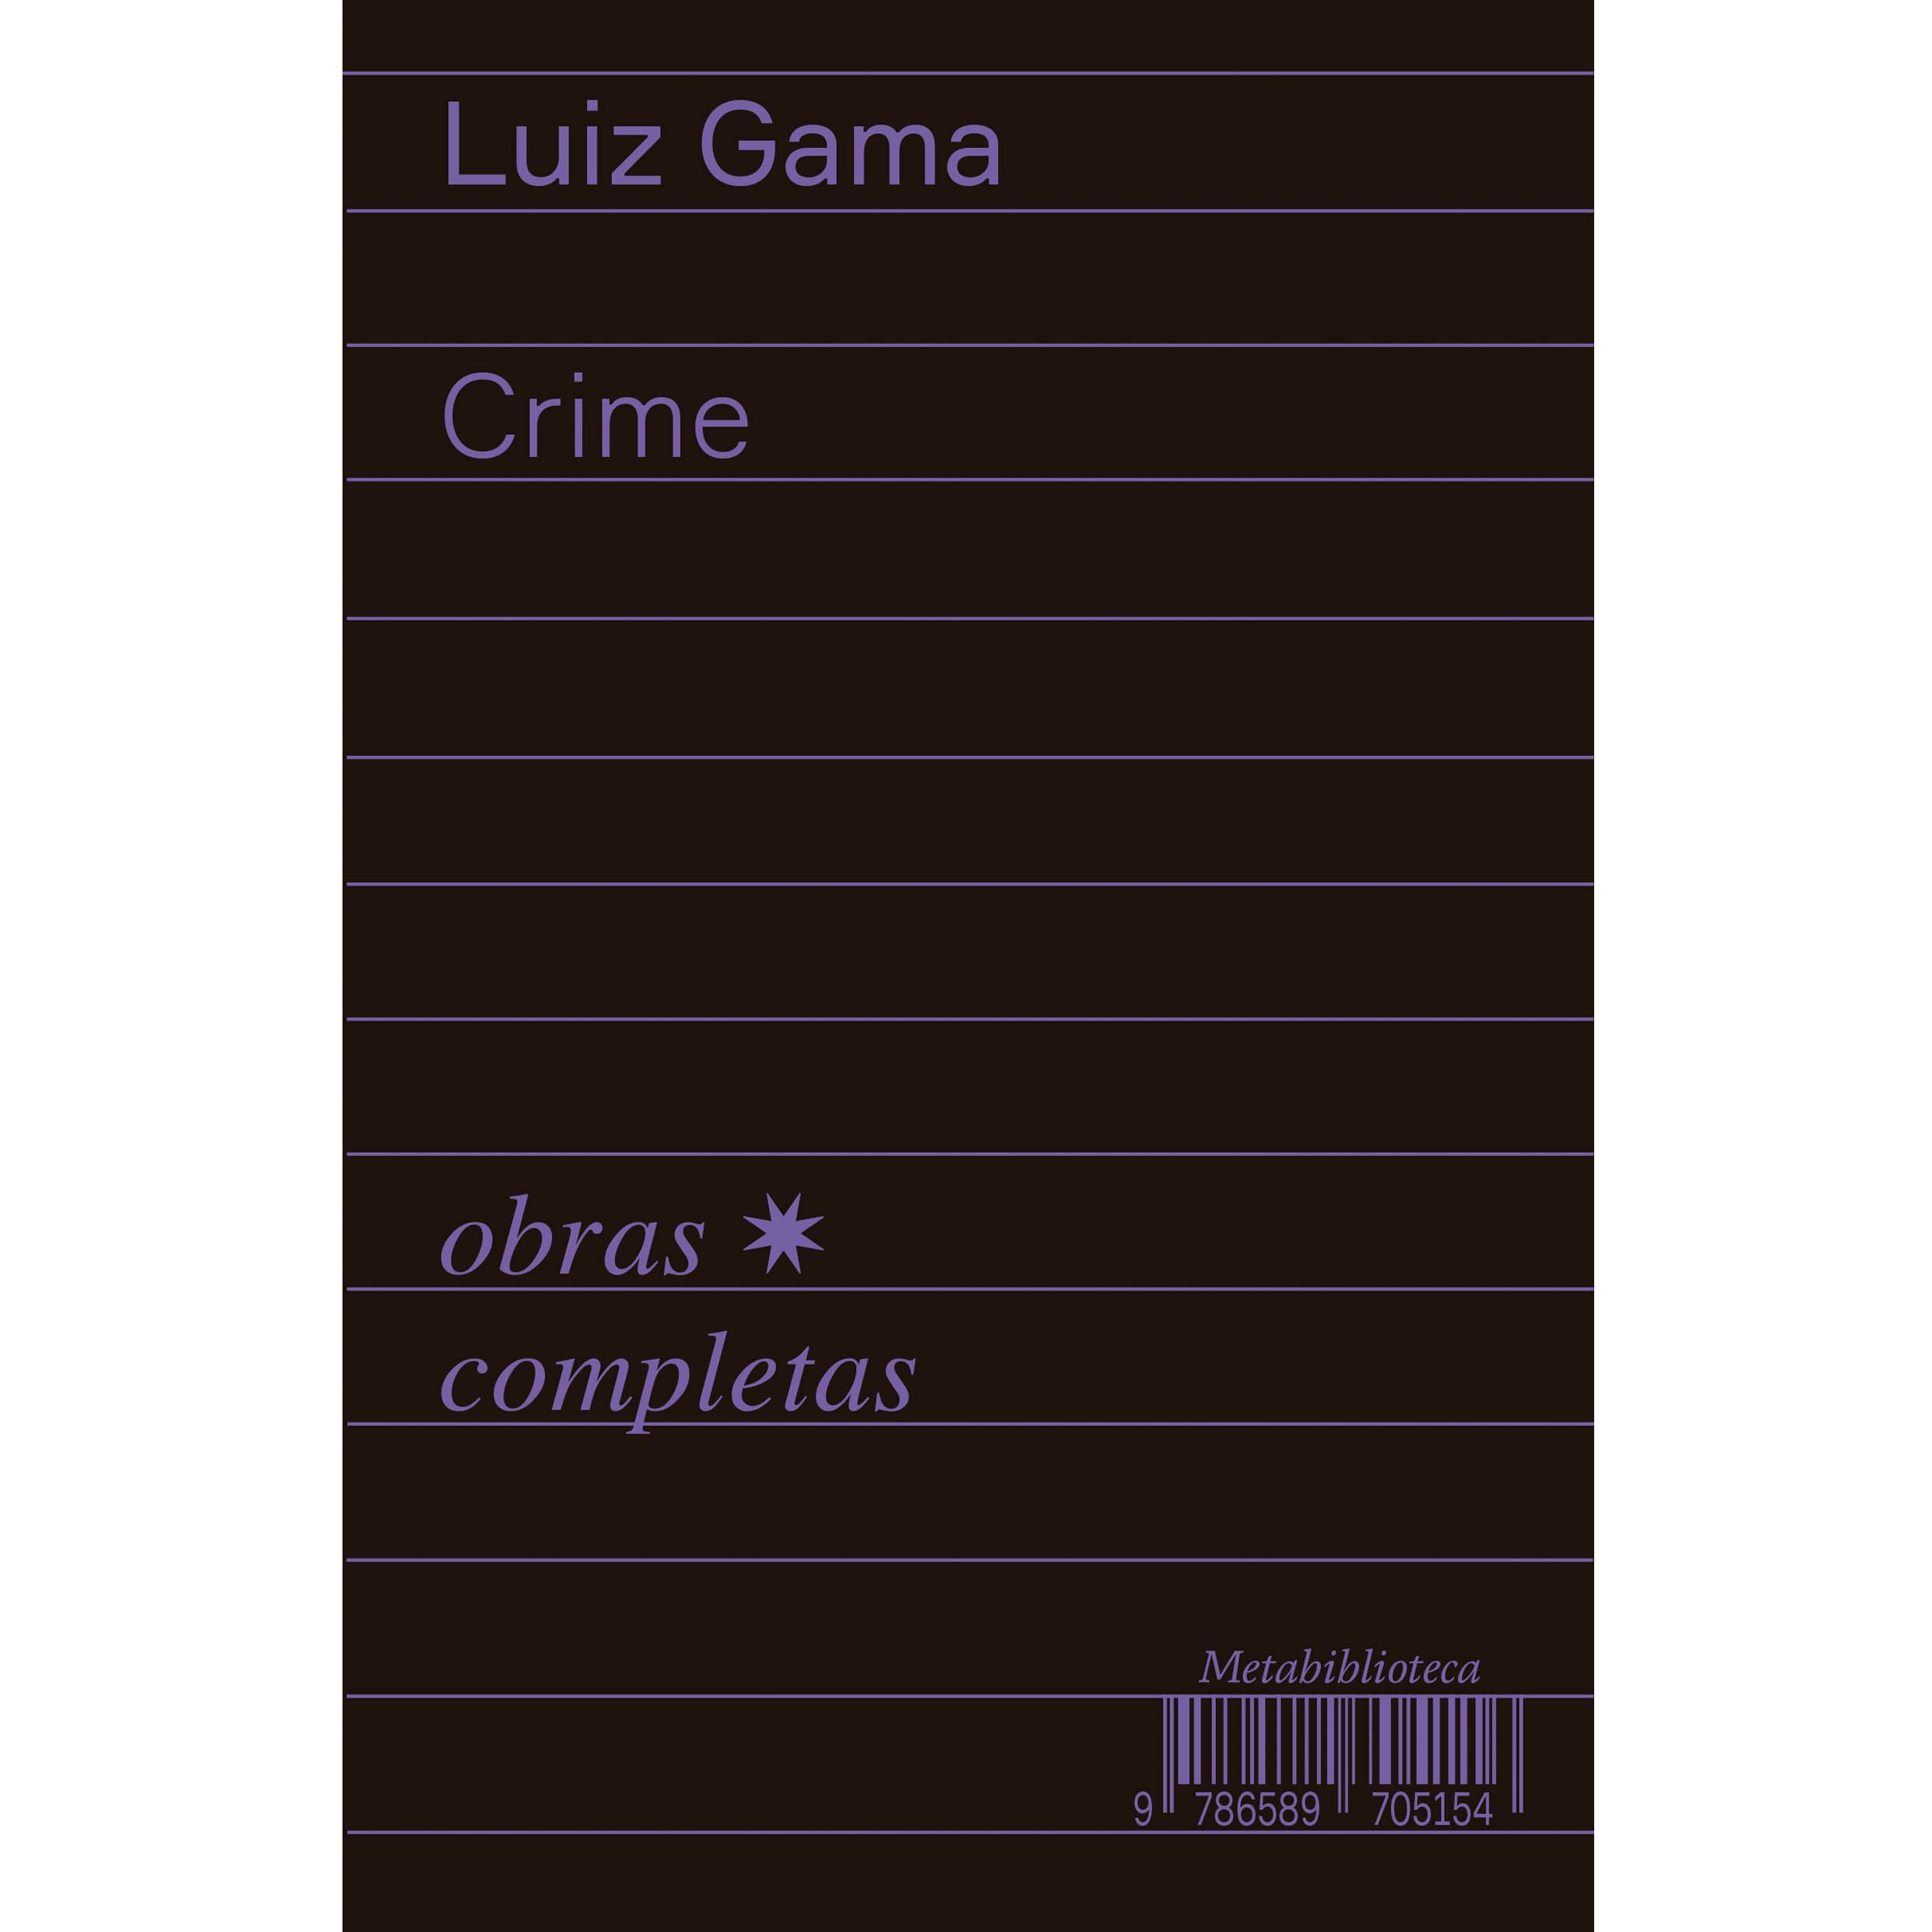
\includegraphics[width=74mm]{./CAPAS/HEDRA_CRIME.jpg}
\end{center}
\hspace*{-7cm}\hrulefill\hspace*{-7cm}
\medskip

\noindent{}\textit{Crime} apresenta \hlc{a volta de Luiz Gama ao direito a partir de textos que são, em sua maioria, casos criminais: petições de \textit{habeas corpus}, denúncias de violação de direitos de presos e prisões ilegais.} E tornam este livro uma espécie de desenvolvimento do quinto volume, \textit{Direito}. Relacionados à matéria penal e processual penal, \textit{Crime} revela o conhecimento de causa com que interpretava o direito criminal do Brasil. Uma habilidade técnica que outros --- que o chamavam \textit{rábula} --- tentam diminuir, ocultar ou desprezar.

\textit{Crime} integra as \textit{Obras completas} de Luiz Gama, advogado negro e abolicionista, a serem lançadas em 11 volumes com cerca de 800 escritos --- 600 inéditos ---, revelando as diversas facetas e estilos empregados pelo escritor para advogar pela grande causa de sua vida: a abolição da escravidão e a emancipação negra. Esquecidos em parte por quase dois séculos, os textos foram recuperados pelo pesquisador Bruno Rodrigues de Lima, que passou nove anos localizando-os em arquivos da imprensa e do judiciário de todo o país.

\vfill
\noindent\begin{minipage}[c]{1\linewidth}
{\small\textbf{
\hspace*{-.1cm}Editora: Hedra\\
Título: Crime [1877--1879]\\
Autor: Luiz Gama\\ 
ISBN: 978-65-89705-15-4\\
Páginas: Inserir.\\
Formato: 13,3x21\,cm\\
Preço: R\$ Inserir.\\
}}
\end{minipage}
\pagebreak

\begin{center}
\hspace*{-3.6cm}\raisebox{5cm}{\rotatebox[origin=t]{90}{\huge\textbf{Lançamento}}}
\hspace*{3.1cm}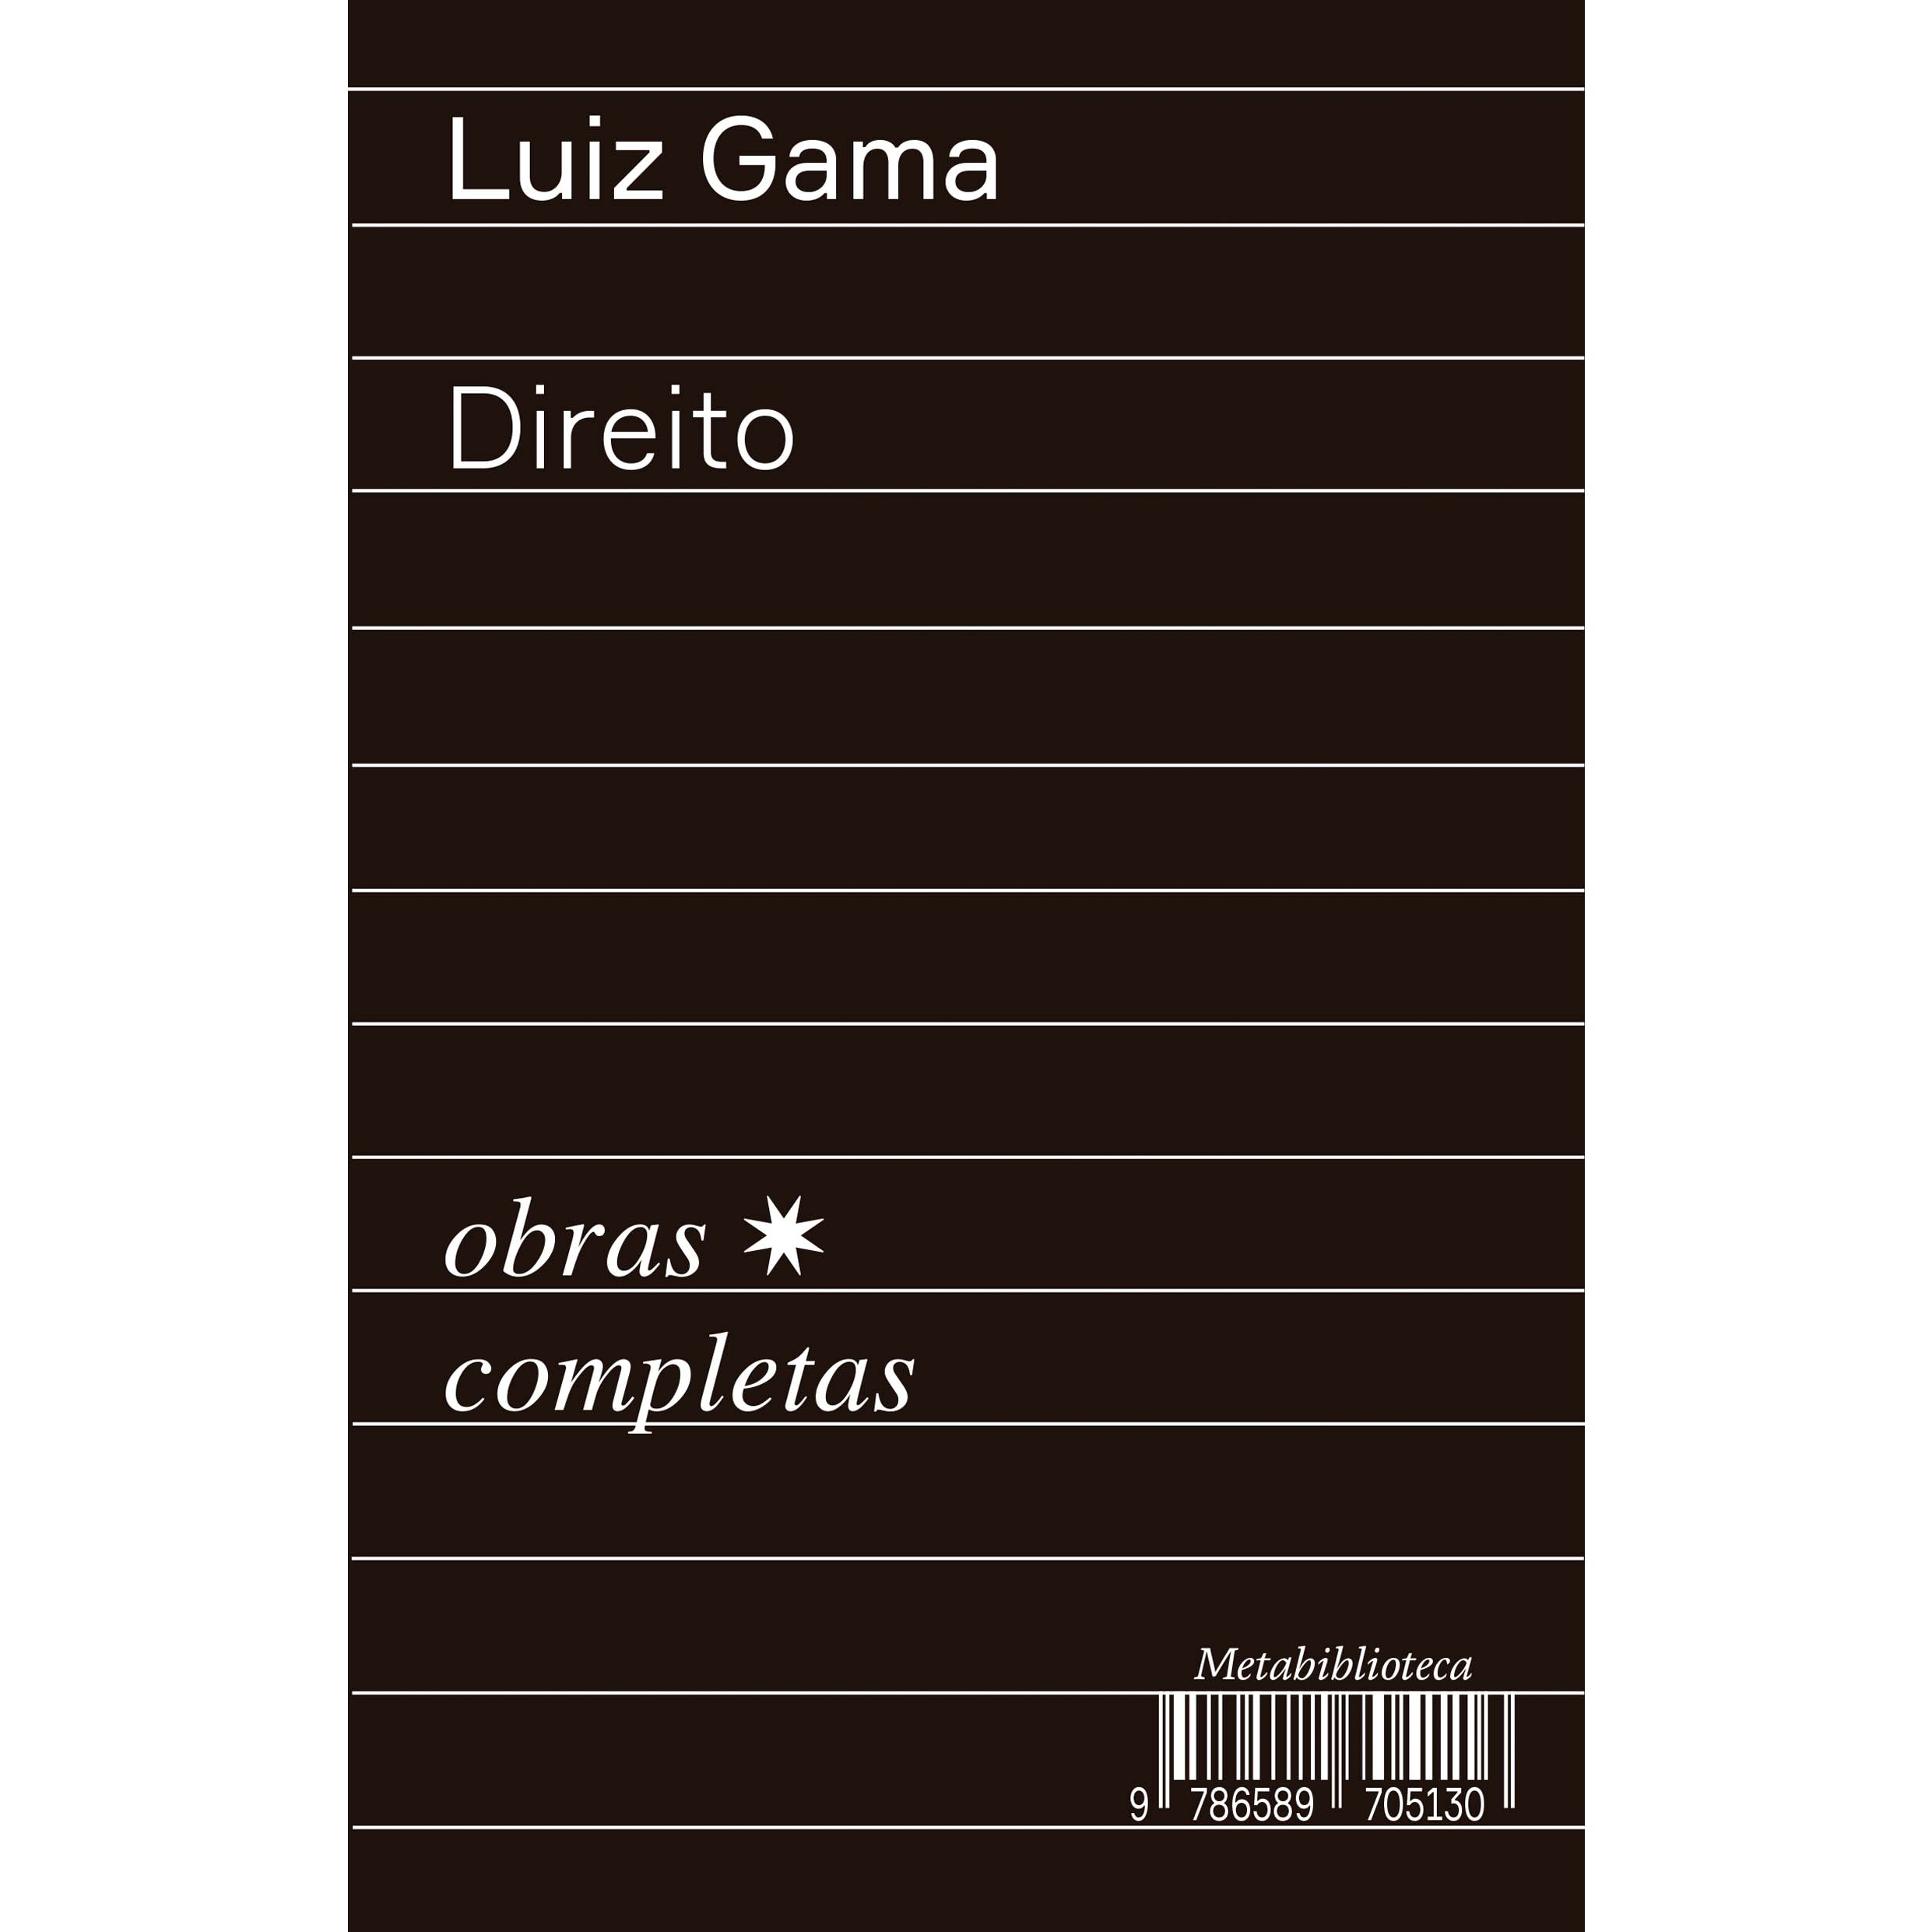
\includegraphics[width=74mm]{./CAPAS/HEDRA_DIREITO.jpg}
\end{center}
\hspace*{-7cm}\hrulefill\hspace*{-7cm}
\medskip

\noindent{}\textit{Direito} é marcado pela saída de Luiz Gama da polícia e o início de seu percurso como advogado. Este volume reúne sua literatura normativo-pragmática: são textos que podem ser lidos segundo divisões temáticas internas do direito e a partir dos casos concretos. \hlc{A maioria dos textos trata de causas que envolvem escravidão e liberdade, mas Gama também atuou em causas de outras naturezas jurídicas}, eminentemente técnicas, sem lidar com a questão da vida e da morte, o que revela o domínio intelectual do advogado.

\textit{Direito} integra as \textit{Obras completas} de Luiz Gama, advogado negro e abolicionista, a serem lançadas em 11 volumes com cerca de 800 escritos --- 600 inéditos ---, revelando as diversas facetas e estilos empregados pelo escritor para advogar pela grande causa de sua vida: a abolição da escravidão e a emancipação negra. Esquecidos em parte por quase dois séculos, os textos foram recuperados pelo pesquisador Bruno Rodrigues de Lima, que passou nove anos localizando-os em arquivos da imprensa e do judiciário de todo o país.

\vfill
\noindent\begin{minipage}[c]{1\linewidth}
{\small\textbf{
\hspace*{-.1cm}Editora: Hedra\\
Título: Direito [1870--1875]\\
Autor: Luiz Gama\\ 
ISBN: 978-65-89705-13-0\\
Páginas: Inserir.\\
Formato: 13,3x21\,cm\\
Preço: R\$ Inserir.\\
}}
\end{minipage}
\pagebreak

\vspace*{1.5cm}
\noindent{}{\nohyphens{\LARGE{Um novo patamar da luta\\política abolicionista}}}
\bigskip

\hfill{}\scalebox{.8}{BRUNO RODRIGUES DE LIMA}
\bigskip
\bigskip
\bigskip

\begin{multicols}{2}
\noindent{}Como Luiz Gama radicalizou a luta abolicionista no Brasil? Quais foram suas táticas de luta --- no debate na imprensa e nos tribunais? Quem esteve ao seu lado a toda 
hora --- e quem atravessou a rua de fininho e mudou de calçada?
O volume \textit{Liberdade} reúne textos que respondem a essas, e outras, perguntas.

Partindo do início de 1880 e chegando até a morte de Gama, em agosto de 1882, \textit{Liberdade} sintetiza a visão política da maior liderança abolicionista de São Paulo na última década da escravidão no Brasil. Jornalista e advogado experiente, Gama usaria de sua veia literária para mudar a chave narrativa e operar uma clivagem conceitual e prática no reposicionamento do movimento abolicionista em São Paulo, que viria a ter repercussão em todo o país. Muito de caso pensado, Gama politizará a racialização da violência e do terrorismo de Estado, radicalizando, assim, o discurso abolicionista a níveis nunca antes vistos. E o fará na esfera discursiva, em momentos decisivos, através de pseudônimos, convertidos em arma retórica e nexo de inflexão radicalizadora do conceito e da prática.

De modo inédito no abolicionismo brasileiro, Gama definiria a política da escravidão como significante indissociável de violência, crueldade, terror, crime e impunidade, ao passo em que enalteceria a resistência dos escravizados pardos e negros como ação política imbuída de indiscutível valor moral e autonomia da vontade.

\vspace{\baselineskip}
{\small\fakereceipt{
\noindent{}Quem abrisse os jornais daquela quarta"-feira, 1º de dezembro de 1880, principalmente no Rio de Janeiro ou em São Paulo, veria que três grandes polêmicas sobre a escravidão tomavam corpo na imprensa. Nas três, a presença do advogado negro Luiz Gama se destacava.
}}
\vspace{\baselineskip}

E Gama dirigia essa radicalização conceitual no abolicionismo com um sentido pragmático: conquistar a abolição e a cidadania ampla, geral e irrestrita o mais rápido possível. Para isso, posicionou o tema da violência racial e policial nos mais improváveis repertórios, como a filosofia do direito natural e o conhecimento normativo legislativo, doutrinário e jurisprudencial brasileiro, descrevendo em mínimos detalhes a estupidez branca e o terrorismo judiciário da política da escravidão.

Parte significativa dos próprios abolicionistas reagiria muito mal à mudança de chave narrativa de Gama. Joaquim Nabuco, por metonímia da classe, diria mais tarde que o seu abolicionismo era o de baluartes como Wilbeforce e Garrisson, e não o “de Spartacus, ou de John Brown”,\footnote{Joaquim Nabuco. \textit{O abolicionismo}. Londres: Tipografia de Abraham Kingdon, 1883, p.\,25.} aqui tomados como signos de fúria e barbárie.

Para bom entendedor, é claro que ele refutava oblíqua e dissimuladamente as ideias de Gama, que dois anos antes escrevera que desejava ser ``louco como Espártacos, como Lincoln, como John Brown, como Jesus''.\footnote{``A liberdade urge'', conforme cita o original.} Se ninguém serve a dois senhores, logo se verá que o abolicionismo de um não foi, e quiçá nunca mesmo poderia ter sido, o abolicionismo do outro.

Assim como o movimento que ele organizava, pode"-se dizer que Gama elegia ``retóricas, estratégias e arenas conforme a conjuntura política''.\footnote{Angela Alonso. \textit{Flores, votos e balas: o movimento abolicionista brasileiro (1868--88)}. São Paulo: Companhia das Letras, 2015, p.\,19.} No início da década de 1880, que lamentavelmente marcaria o final de sua vida, o advogado  mudava o patamar discursivo do abolicionismo no espaço público brasileiro, escolhendo a retórica da fúria negra, potencializada pelo uso de pseudônimos enquanto estratégia autoral, para disseminar sua voz por diferentes arenas de debates, sempre atento às injunções da conjuntura política --- sobretudo a da política local. A combinação explosiva desses elementos atordoaria correligionários, oponentes e inimigos. Mas inegavelmente representava a esperança de liberdade, justiça e cidadania para ``um milhão e quinhentas mil vítimas do mais abominável crime''.\footnote{``Terrorismo judiciário'', conforme cita o original.}

O Brasil de 1880 estava numa encruzilhada --- e Gama não tinha dúvida de que lado, e ao lado de quem, estava.

Quem abrisse os jornais daquela quarta"-feira, 1º de dezembro de 1880, principalmente no Rio de Janeiro ou em São Paulo, veria que três grandes polêmicas sobre a escravidão tomavam corpo na imprensa. Nas três, a presença do advogado negro Luiz Gama se destacava. Na capa da \textit{Gazeta da Tarde}, folha carioca de viés abolicionista, aparecia o despretensioso ``trecho de uma carta'' que, como se confirmaria nos meses seguintes, seria a primeira das onze partes de uma das mais impressionantes, senão a mais radical obra política de Luiz Gama.\footnote{``Olho vivo no parlamento'', conforme cita o original.} 

Em São Paulo, onde conhecia a todos e era por todos conhecido, outros dois artigos ganharam as páginas naquele mesmo dia: um na \textit{Gazeta do Povo}, em que, defendendo o seu camarada José do Patrocínio, anunciava um novo patamar da luta política abolicionista;\footnote{``O meu companheiro José do Patrocinio'', conforme cita o original.} e outro artigo na \textit{Província de S.\,Paulo} que, como se verá, teve de usar de um pseudônimo para denunciar a tortura e o assassinato de uma criança parda de sete anos de idade pelas mãos de dois senhores brancos, que a quiseram enterrar viva.\footnote{``Revirando as vísceras da medicina legal'', conforme cita o original.}

Os três artigos não foram, até hoje, lidos em conjunto. Trata"-se, portanto, de reunião inédita na literatura de Luiz Gama. Partes de uma mesma estratégia literária e editorial, os três artigos abrem portas para se compreender a obra do maior jurista da história desse país e a sua luta, com as roupas e as armas da imprensa e do direito, pela liberdade e pelos direitos dos humilhados, ofendidos e condenados da terra. Semelhantes no propósito, os três artigos, contudo, tinham formas e destinatários diferentes, o que explica terem sido publicados não em um, mas em três jornais distintos. Com isso, intensificava a presença abolicionista na imprensa, visando, certamente, acelerar o processo histórico em curso.

Na capital do Império, Gama era apresentado pela \textit{Gazeta da Tarde} como o maior líder abolicionista em São Paulo. Desse lugar, ele se dirigia ao público simpático às ideias que tinham em comum, mirando um movimento popular de massas que derrubasse a monarquia, que ele entendia ser a fonte de sustentação da escravidão. Suas cartas corriam no fio da navalha, entre a sobriedade do jurista erudito e a insurgência do revolucionário, emitindo múltiplas mensagens para a diversidade de atores na arena política, muito embora tivessem o objetivo prático de mobilizar os abolicionistas para um conjunto de ações em comum. Foi justamente nesse contexto, como reforço à construção de sua liderança junto ao movimento, agora em perspectiva nacional, que a \textit{Gazeta da Tarde} publicou seu perfil biográfico, destacando pela primeira vez a jornada épica do menino preto nascido livre, escravizado pelo próprio pai, que fugiu do cativeiro e conquistou sua liberdade para, no futuro, libertar mais de quinhentas pessoas ilegalmente escravizadas.

\bigskip
\noindent{}\textcolor{gray}{\footnotesize\slsc{\textls[-15]{Excerto da introdução do volume ``Liberdade'', oitavo volume das \textit{Obras completas} de Luiz Gama.}}}
\end{multicols}

\pagebreak
\pagestyle{hedracat}
\begin{multicols}{2}
\begin{enumerate}
\raggedright\nohyphens{
\item Teogonia \textbf{Hesíodo}
\item O ladrão honesto e outros contos \textbf{Fiódor Dostoiévski}
\item Micromegas \textbf{Voltaire}
\item A sociedade de controle \textbf{Joyce Souza; Rodolfo Avelino; Sérgio Amadeu da Silveira}
\item O quarto poder \textbf{Paulo Henrique Amorim}
\item Deus e o Estado \textbf{Mikhail Bakunin}
\item Lugar de negro, lugar de branco? \textbf{Douglas Rodrigues Barros}
\item O princípio anarquista e outros ensaios \textbf{Piotr Alekseievitch Kropotkin}
\item Dicionário de história e cultura da era viking \textbf{Johnni Langer}
\item Poesia completa \textbf{Orides Fontela}
\item Sobre verdade e mentira \textbf{Friedrich Nietzsche}
\item Dicionário de mitologia nórdica \textbf{Johnni Langer}
\item Rashômon e outros contos \textbf{Akutagawa}
\item O indivíduo, a sociedade e o Estado e outros ensaios \textbf{Emma Goldman}
\item Memórias do subsolo \textbf{Fiódor Dostoiévski; Lucas Simone}
\item O chamado de Cthulhu \textbf{H. P. Lovecraft}
\item Bom crioulo \textbf{Adolfo Caminha; João Silvério Trevisan}
\item Nos cumes do desespero \textbf{Emil Cioran}
\item Édipo Rei \textbf{Sófocles}
\item Dilma Rousseff e o ódio político \textbf{Tales Sáber}
\item Contos clássicos de vampiro \textbf{Lord Byron; Bram Stoker}
\item Trabalhos e os dias \textbf{Hesíodo}
\item Sobre a utilidade e a desvantagem da história para a vida \textbf{Friedrich Nietzsche}
\item Saga dos volsungos \textbf{Anônimo}
\item O contador de histórias \textbf{Walter Benjamin; Patrícia Lavelle; Georg Otte; Marcelo Backes; Patrícia Lavelle; Amon Pinho; Francisco Machado}
\item Michel Temer e o fascismo comum \textbf{Tales Ab'Sáber}
\item A metamorfose \textbf{Franz Kafka}
\item A filosofia na era trágica dos gregos \textbf{Friedrich Nietzsche}
\item O médico e o monstro \textbf{Robert Louis Stevenson}
\item Diário de um escritor (1873) \textbf{Fiódor Dostoiévski}
}
\end{enumerate}
\end{multicols}

\pagebreak
